\documentclass[12pt, letterpaper]{article}
\usepackage[titletoc,title]{appendix}
\usepackage{color}
\usepackage{booktabs}
\usepackage[usenames,dvipsnames,svgnames,table]{xcolor}
\definecolor{dark-red}{rgb}{0.75,0.10,0.10}
\definecolor{bluish}{rgb}{0.05,0.05,0.85}

\usepackage[margin=1in]{geometry}
\usepackage[linkcolor=blue,
			colorlinks=true,
			urlcolor=blue,
			pdfstartview={XYZ null null 1.00},
			pdfpagemode=UseNone,
			citecolor={bluish},
			pdftitle={partisan_gap}]{hyperref}

\usepackage[resetlabels,labeled]{multibib}
\newcites{SI}{SI References}
\usepackage{natbib}

\usepackage{float}

\usepackage{geometry} % see geometry.pdf on how to lay out the page. There's lots.
\geometry{letterpaper}               % This is 8.5x11 paper. Options are a4paper or a5paper or other... 
\usepackage{graphicx}                % Handles inclusion of major graphics formats and allows use of 
\usepackage{amsfonts,amssymb,amsbsy}
\usepackage{amsxtra}
\usepackage{verbatim}
\setcitestyle{round,semicolon,aysep={},yysep={;}}
\usepackage{setspace}		     % Permits line spacing control. Options are \doublespacing, \onehalfspace
\usepackage{sectsty}		     % Permits control of section header styles
\usepackage{pdflscape}
\usepackage{fancyhdr}		     % Permits header customization. See header section below.
\usepackage{url}                     % Correctly formats URLs with the \url{} tag
\usepackage{fullpage}		%1-inch margins
\usepackage{multirow}
\usepackage{rotating}
\setlength{\parindent}{3em}

\usepackage[T1]{fontenc}
\usepackage[bitstream-charter]{mathdesign}

\usepackage{chngcntr}
\usepackage{booktabs}
\usepackage{longtable}

\def\citeapos#1{\citeauthor{#1}'s (\citeyear{#1})}

\makeatother

\usepackage{footmisc}
\setlength{\footnotesep}{\baselineskip}
\makeatother
\renewcommand{\footnotelayout}{\normalsize \doublespacing}


% Caption
\usepackage[hang, font=small,skip=0pt, labelfont={bf}]{caption}
%\captionsetup[subtable]{font=small,skip=0pt}
\usepackage{subcaption}

% tt font issues
% \renewcommand*{\ttdefault}{qcr}
\renewcommand{\ttdefault}{pcr}

\setcounter{page}{0}

\usepackage{lscape}
\renewcommand{\textfraction}{0}
\renewcommand{\topfraction}{0.95}
\renewcommand{\bottomfraction}{0.95}
\renewcommand{\floatpagefraction}{0.40}
\setcounter{totalnumber}{5}
\makeatletter
\providecommand\phantomcaption{\caption@refstepcounter\@captype}
\makeatother

\title{A Gap in Our Understanding? Reconsidering the Evidence for Partisan Knowledge Gaps\footnote{We are grateful to Doug Ahler, John Bullock, Hans Hassell, Don Green, Andy Guess, Matt Pietryka, and participants in the Democracy Fellows Seminar at the Ash Center for Democratic Governance and Innovation at the Harvard Kennedy School for their helpful comments and suggestions. A previous version of this paper was presented at the 2020 Annual Meeting of the Southern Political Science Association.}}

\author{Carolyn E. Roush\thanks{Corresponding author, Visiting Assistant Professor of Political Science, Florida State University, \href{mailto:croush@fsu.edu}{\texttt{croush@fsu.edu}}} \and Gaurav Sood\thanks{Independent researcher, \href{mailto:gsood07@gmail.com}{\texttt{gsood07@gmail.com}}}}


\begin{comment}

setwd(paste0(githubdir, "partisan_gap/ms/"))
tools::texi2dvi("partisan_gap_gs.tex", pdf = TRUE, clean = TRUE)
setwd(githubdir)

\end{comment}

\begin{document}
\maketitle
\thispagestyle{empty}

\begin{abstract}

\noindent Conventional wisdom suggests large, persistent gaps between partisans' stores of political knowledge, fanning concerns about democratic accountability. We reconsider the frequency and size of these ``partisan knowledge gaps,'' assembling a dataset of 162,083 responses to 187 items on 47 surveys. We find these gaps are smaller and less frequent than commonly understood; the average is a mere six points and gaps' ``signs'' run counter to expectations roughly 30\% of the time. Additionally, while most question features fail to predict gap size, we find that questions featuring vague response options allow individuals to interpret potential answers through their own biases, inflating gaps' magnitudes. Our findings suggest that knowledge gaps---when they do exist---stem more from motivated responding than genuine differences in factual knowledge.

\end{abstract}

\vspace{.2in}

\newpage

\doublespacing

Factual knowledge about politics has long been viewed by scholars as key to democratic competence. Higher levels of political knowledge correspond to a number of normatively desirable outcomes, including higher levels of political tolerance and support for democratic norms, more active participation in politics, and more stable and consistent opinions on political matters \citep{Converse1964,dellicarpini,galston_2001}. Political knowledge also helps facilitate connections between individual group identities and policy views, which can then be applied to evaluations of public officials and parties in a way that increases democratic accountability \citep{dellicarpini}.

Political knowledge's centrality to democratic health is perhaps why so many are troubled by the fact that Democrats and Republicans appear to differ in their knowledge of politics. Partisans' biased interpretation and retention of political facts appears in public opinion data reaching at least as far back as the 1980s \citep[e.g.,][]{bartels_2002,jerit2012partisan}. As such, the idea of large partisan knowledge gaps---differences in the types of information that Democrats and Republicans know---has become axiomatic in the political science. Indeed, as \citet{bullocketal_2015} note, conventional wisdom in the discipline that ``a persistent pattern in American public opinion is the presence of large differences between Democrats and Republicans in statements of factual beliefs'' (520). Everyday Americans seem to be catching on as well. A poll conducted by the Pew Research Center in 2018 demonstated that nearly eight in ten Americans believe that Democrats and Republicans not only disagree on plans and policies, but on facts as well \citep{pew2018disagree}. 

Large knowledge gaps stemming from partisan biases are concerning. Just as high levels of political knowledge can lead to better citizenship, mass disagreement politically consequential facts can impede democratic governance and representation. Theories of retrospective accountability hinge citizens' ability to judge how well incumbents have performed in office  \citep{fiorina1981retrospective,Key1966,kramer_1971}. If Republicans and Democrats rely upon different sets of facts to make these judgments, elected officials have weaker incentives to work for their constituents. Partisan disagreement about basic facts also reduces the possibility of meaningful dialogue. If Republicans and Democrats disagree about how the economy is doing, a discussion about policies for improving the economy is unlikely to follow. 

Given the long shadow that these gaps cast on the health of democracy, understanding how often and to what extent partisans differ in their knowledge of political facts is vital. To study the issue, we assembled a large dataset of partisan-relevant knowledge items. To do so, we made use of data from three prominent studies on the nature and pervasiveness of partisan knowledge gaps \citep{bullocketal_2015,jerit2012partisan,prior2015you}. We find that partisan knowledge gaps are highly variable, and that large differences in what Democrats and Republicans believe are less common than conventional wisdom suggests. In fact, fewer than one in three partisan knowledge gaps are larger than ten percentage points. In addition, nearly one in three partisan knowledge gaps are in the ``wrong'' direction, that is, partisans know less party-congenial information than their opponents. In addition, more than half of the gaps in the expected direction are not statistically significant at conventional levels, despite large sample sizes. On the whole, the average knowledge gap between Democrats and Republicans is six percentage points.

We attempt to reconcile these findings with the conventional wisdom that partisan knowledge gaps are large and pervasive. We find little evidence that features of question wording systematically affect the size of such gaps; only questions that ask about topics about which there is significant misinformation or questions that are asked during presidential election campaigns appear to meaningfully influence the size of such gaps. We do, find, however, that the wording of response options matters. Specifically, we find that much of the conventional wisdom surrounding the ubiquity and size of knowledge gaps can be traced to  \citet{anes_gen} (ANES) questions, which include vague response options that encourage respondents to interpret meaning based on their own partisan biases. In a companion paper, using an original experiment, we demonstrate that vague response options of this type can produce partisan knowledge gaps \textit{even when} Democrats and Republicans know the answer \citep{roush_2021}. Taken together, our results support the conclusion that partisan knowledge gaps---when they do exist---are more an artifact of ``partisan cheerleading'' \citep{bullocketal_2015,prior2015you} or motivated guessing than a reflection of genuine differences in knowledge.


\section*{Partisan Learning and Political Knowledge}

During Bill Clinton's first term as president, the US budget deficit shrunk from \$255 billion to \$22 billion. Near the end of 1996, when the ANES asked a representative sample of Americans whether the budget deficit had decreased, increased, or remained the same over the past four years, far fewer Republicans than Democrats knew that the deficit had declined. While 39\% of Democrats correctly identified that the budget deficit had decreased, only 25\% of Republicans did the same \citep[280]{achen2016democracy}.

Such large discrepancies are considered neither anomalous nor unexpected. Our understanding of how partisan bias influences information processing suggests that there are good reasons to expect partisan knowledge gaps to be large and ubiquitous. The psychological processes underlying the development of knowledge gaps is similar to those that produce partisan differences in attitudes and evaluations on a wide variety of subjects. When people encounter information that conflicts with their predispositions, they experience cognitive discomfort, which they try to minimize by employing a variety of defense mechanisms \citep[e.g.,][]{abelson1959modes,festinger1962theory}. Specifically, they avoid exposing themselves to sources that provide them with uncongenial information, distrust such information when they do come across it, and do not work as hard to retain it \citep{bartels_2002, jerit2012partisan, lodgetaber_2013}. Partisanship helps reduce cognitive discomfort by acting as a ``perceptual screen,'' filtering in congenial facts that comport with an individual's partisan worldview while filtering out those that challenge it \citep{campbell1960, Zaller1992}. As a result, the theory goes, Democrats and Republicans come to ``know'' different types of information and consequently vary in their ability to answer political knowledge questions correctly.

That being said, recent scholarship has provided reasons to doubt that these knowledge gaps are as frequent and sizable as commonly believed. For one,  \citet{bullocketal_2015} and \citet{prior2015you} demonstrate that partisan gaps in factual beliefs about politics are often the product of motivated responding. ``Partisan cheerleading'' arises when partisans want to send a message to either pollsters or the public at large about the strength or righteousness of their preferred party's stance on a particular matter \citep{huber_yair_2018}. As a result, what may look like differences in political knowledge among partisans may be more a consequence of respondents providing party-congenial responses rather than expressing what they genuinely know. \citet{bullocketal_2015} and \citet{prior2015you} show that these partisan gaps can be reduced by shifting respondents' directional motives to accuracy motives via small monetary incentives for correct answers. More recently, \citet{huber_yair_2018} also showed that partisan gaps shrink when survey respondents are given the opportunity to cheerlead prior to answering other questions. Taken together, these studies suggest that the concern that Democrats and Republicans are truly drawing on differential bases of political knowledge may be overblown.

Secondly, a more critical examination of the processes thought to underlie the production of knowledge gaps suggests that genuine differences in knowledge between Democrats and Republicans should be smaller. According to the theory of selective exposure, Democrats and Republicans consume different media sources, thereby learning and retaining different facts that are reflected in reported knowledge of political information \citep[e.g.,][]{Stroud2008,stroud_2010}. In reality, however, most people consume very little political news \citep{Prior2007,flaxmanetal_2016}, and the news that they do consume is relatively ideologically balanced \citep{flaxmanetal_2016,garzetal_2018,gentzkowshapiro_2011,guess_2020}. There is little reason, therefore, to believe that knowledge gaps emerge as a result of partisans simply tuning into different sources. Regardless of where partisans get their information, evidence shows that they do learn facts in a motivated fashion \citep{hill_2017,jerit2012partisan,khanna2018motivated}---but the effects are modest, and people exhibit little partisan bias in their recall of information \citep{khanna2018motivated}. Other scholars have pointed out that Democrats and Republicans respond to current events in a similar fashion, bringing into question the existence of motivated learning in the first place \citep{gerber_annual_review,kernell_2019}. Therefore, the conventional wisdom regarding the individual-level mechanisms thought to produce large knowledge gaps may be flawed.

Given what scholars know about the nature of partisan survey response, news consumption, and knowledge recall, there are good reasons to doubt that partisan knowledge gaps are as large, ubiquitous, and normatively troubling as expected. That being said, we lack a comprehensive understanding of the nature and frequency of such partisan differences outside of experimental contexts. Indeed, as \citet{bullocklenz_2019} note in their review of partisan bias in surveys, ``despite burgeoning interest in partisan differences [in responses to factual questions about politics], there have been few attempts to generalize about the size of these differences'' (330).  In the remainder of this paper, we attempt to do just that.

\section*{Data and Research Design}

To estimate the frequency and size of partisan knowledge gaps, we assembled a large dataset of political knowledge items. Because we are interested in the degree to which partisan reasoning produces knowledge gaps, we focused on questions about partisan-relevant facts---that is, facts that carry ``positive or negative implications for one's party'' \citep[][673]{jerit2012partisan} that have an objectively correct answer.

To build the dataset, we harvested data from three prominent studies on partisan knowledge gaps. The first two studies---\citet{bullocketal_2015} and \citet{prior2015you}---use survey experiments to estimate the degree to which partisan knowledge gaps are a product of expressive responding. In our current study, however, we are interested in measuring the extent to which partisan gaps exist on ordinary public opinion surveys, regardless of the process by which they are generated. Accordingly, we only used data from the control group of these studies. A third study from which we source data focuses on explaining partisan gaps and includes both observational and experimental data \citep{jerit2012partisan}. Here, we only used data from the observational study---which compiles questions from surveys conducted by national news organizations---as the experiment focuses on partisan learning, not on gaps in stored knowledge. 

In addition, we also compiled all knowledge items that carry a partisan implication that appeared on the \citet{anes_gen} (ANES) over the past 32 years.\footnote{For reasons of subjectivity, we excluded questions that asked respondents to assess how ``the economy'' has fared. While many response options to questions on the ANES are vague, in this case, the question itself asks respondents to evaluate a vague concept (the economy) as well. That is, answers to these types of questions hinge on both what survey respondents think ``the economy'' means and on what they think is a good indicator of its health. For example, in answering a question about how ``the economy'' did over the previous year, some respondents may read the question as asking about their state or local economy, while others may reference the unemployment rate, changes in their disposable income, or (among the highly knowledgeable) the performance of the stock market. While some political scientists have attached their own metrics, like real disposable income per capita \citep[e.g.,][]{achen2016democracy,hibbs2000}, to ``objectively'' gauge how the economy is doing, many survey respondents will plausibly differ in their reference points. Nevertheless, in \ref{append_econ}, we track partisan gaps in economic evaluations. As expected, there are much larger differences between Democrats and Republicans in their assessments of ``the economy'' compared to other knowledge items. These items produce an average gap of 17.2 percentage points.}  To gauge partisans' accuracy on these items, we identified ``correct'' responses based on information sourced from federal agencies like the Bureau of Labor Statistics, the Federal Reserve, and the Census Bureau, in addition to information gleaned from news reporting or academic studies.\footnote{For the same reasons mentioned above, identifying which response option is ``correct'' requires some level of subjectivity. As we detail in \ref{si:q_text}, for the purposes of this exercise, we applied a consistent standard across the board: we classify changes in performance indicators as ``stayed about the same'' unless the change exceeds one third of one percentage point in either direction.} As before, we dichotomized response options into ``correct'' and ``incorrect'' categories. Like the authors in the other studies, we also assumed that there is no ``hidden knowledge'' behind ``don't know'' responses and code them as incorrect \citep{luskin2011don}.\footnote{\citet{luskin2011don} estimate proportion of ``hidden knowledge'' in ``don't know'' responses to be only about 3\%, suggesting that we are not substantially underestimating political knowledge by coding ``don't knows'' as incorrect.} 

Altogether, our final dataset includes 162,083 responses to 187 political knowledge items on 47 surveys conducted between 1986 and 2016. The knowledge items cover a range of topics, including how much unemployment increased or decreased over a certain period to how many people died in the Iraq War to whether or not global warming is anthropogenic. For a full list of items along with question-wording and response options, please see Appendix \ref{si:q_text}.\footnote{We omit from our study three placebo questions from \citet{bullocketal_2015} relating to the price of gold in 1980, the Bangladeshi independence date, and the number of Mickey Mantle's home runs in 1961, since none of these questions carry a partisan implication.}\footnote{We also omit two questions from \citet{jerit2012partisan} concerning Iraq's possession of weapons of mass destruction. We do so because the authors' coding indicated that the correct answer was that Iraq ``currently ha[d] weapons'' of mass destruction. However, according to multiple sources--- most notably the CIA---``Iraq's [weapons of mass destruction (WMD)] capability...was essentially destroyed in 1991,'' and it had not acquired or built new WMD between 1991 and 2003, and that WMD ``were not there'' at the time of the U.S.-led invasion in 2003. Futhermore, ``Iraq unilaterally destroyed its undeclared chemical weapons stockpile in 1991...there are no credible indications that Baghdad resumed production of chemical munitions thereafter'' \citep{cia_2004}. In addition, the majority of Iraq's biological weapons had been destroyed in 1991, and there is no credible indication that Iraq resumed the production of biological weapons afterwards \citep{cia_2004}. Due to the nature of \citet{jerit2012partisan}'s replication data, we are unable to correct the coding to reflect the correct answers. Accordingly, we choose not to include these questions in our dataset.}

To determine differences in what partisans know, we took the difference between the proportions of Democrats and Republicans who answered each knowledge question correctly. We followed the authors' coding schemes to dichotomize response options into ``correct'' and ``incorrect'' responses.\footnote{For data sourced from \citet{bullocketal_2015} and \citet{prior2015you}, we followed convention and grouped together leaning Independents with partisans, as research shows that leaners behave and think much like other partisans \citep{keithetal_1992}. Unfortunately, the \citet{jerit2012partisan} data excludes these leaning Independents, instead focusing on knowledge gaps only among individuals who were willing to identify as Democrats or Republicans in response to the traditional three-pronged party identification question. Our results do not change substantially when we exclude leaners from all analyses. Doing so produces a mean gap of 6.2 percentage points, a median gap of 4.6, and a standard deviation of 12.4.} A partisan knowledge gap, then, is defined as the absolute value of the difference between the proportions of Republicans and Democrats who answered a question correctly.

If we use the absolute difference between correct answers among Democrats and Republicans as a measure of knowledge gaps, however, we cannot discern whether the gap is the result of partisans knowing more or less party-congenial information than their opponents. For example, the absolute value of a partisan gap of 14 percentage points produced by a question about the change in the budget deficit under President Clinton could mean that Democrats were more accurate than Republicans \textit{or} that Republicans were more accurate than Democrats. The distinction is an important one, as previous work suggests that knowledge gaps are likely produced by partisans' tendency to more easily learn and retain information that benefits their party and reject or forget information that paints their party in a less-than-favorable light \citep{jerit2012partisan}. Given that the budget deficit sharply declined when Clinton was in office, we expect more Democrats than Republicans to be aware of this information \citep{jerit2012partisan}. A finding that more Republicans than Democrats knew that the budget deficit declined under Clinton would therefore run counter to our understanding of how knowledge gaps are produced. 

Therefore, to better ascertain the nature of partisan knowledge gaps, we imputed the ``sign'' of the gap for each question in our dataset.\footnote{We later discuss our results using the absolute value of the partisan gap.} To do so, we first categorized questions into groups based on question features that should influence the expected sign of each gap. The first and most common group contains questions based on performance. As mentioned above, previous research demonstrates that partisans tend to be more accurate than their opponents when responding to questions that have positive implications for their own party \citep{jerit2012partisan}. Quite often, these positive implications arise when outcomes that are universally desirable---for example, lower unemployment, lower inflation, fewer casualties in foreign wars, lower gas prices, lower taxes, etc.---can be attributed to a co-partisan president. Given how much presidents dominate the news \citep{hopkins2018increasingly} and the imagination \citep{jacobson_2019}, partisans should be more likely than their opponents to know positive things that happen under a co-partisan president. One classic example of this phenomenon is highlighted by \citet{bartels_2002}, who noted that, in 1988, Republicans were more accurate than Democrats in their responses to questions about unemployment and inflation rates, as both decreased during President Reagan's administration (134). In this case, because Republicans were more accurate more about a party-congenial fact than Democrats, we code the sign on the partisan gap as positive. 

Similarly, because partisan politics often plays out as a zero-sum game \citep[e.g.,][]{lee_2016}, we expect partisans to be more accurate about facts that have \textit{negative} implications for their opponents.\footnote{This is especially likely given the rise of negative partisanship and the centrality of out-party feelings to several aspects of public opinion over the past few years \citep[e.g.,][]{abramowitzwebster_2016,hetheringtonrudolph_2015,IyengarSoodLelkes2012,mason_2018,nicholson_2012}.} For example, we expect Democrats to be more informed than Republicans about the change in the unemployment rate if unemployment substantially increased under a Republican president, as it did, for example, between 2000 and 2008 under President George W. Bush. In our data, we code gaps that conform to these expectations as positive.\footnote{Here, we depart from \citet{jerit2012partisan}, which differentiates between items that have positive implications for Democrats, negative implications for Democrats, positive implications for Republicans, and negative implications for Republicans. For the purposes of our analysis, we combine Democratic-positive/Republican-negative and Republican-positive/Democratic-negative. With the exception of collapsing these two categories, however, we rely on the authors' coding of the partisan implication (in other words, the expected sign of the gap) for each item. For this reason, our results differ from \citet{jerit2012partisan}, as our estimand differs: \citet{jerit2012partisan} are interested in calculating differences \textit{across} question items and across people \textit{within the same party}, while we calculate differences \textit{within} items across people \textit{in different parties}.} Conversely, we code gaps that do \textit{not} conform to expectations---that is, those instances in which partisans are \textit{less} accurate about party-congenial facts or \textit{more} accurate about party-\textit{un}congenial facts than their opponents---as negative, as they occur in the ``wrong'' direction. For items for which the partisan implications are debatable---for example, if the unemployment rate stayed more or less the same over the past year---we opt for the conservative option of retaining the absolute value of the partisan gap. In other words, we code partisan gaps in these ambiguous cases as positive; as a consequence, our results are biased in favor of finding large gaps. 

The second category features questions that bear partisan implications that do not hinge on performance. For example, some facts could be considered positive for one set of partisans because their favored party takes action on a particular fact. For example, Democratic environmental policy is based on the (correct) notion that global warming is real and its cause is man-made. Republican policy, on the other hand, is based on the (incorrect) belief that global warming has probably not been happening, and if it has, it is the result of natural causes. On questions related to the existence and source of global warming, therefore, we expect Democrats to know more. Another prominent example relates to the estate tax. In this case, Democratic policy pivots off the fact that a very small proportion of Americans pay estate taxes, while Republican policy is based off the (incorrect) notion that considerably more Americans would be subject to the tax. Again, we expect Democrats to be more accurate than Republicans on questions related to the percentage of Americans subject to an estate tax.

Finally, in a handful of cases, question wording and response options influence the partisan implication of a particular question. For example, in \citet{bullocketal_2015}, a question about the total casualties in Iraq from 2003 to 2008 provides four response options. The correct answer to the question---4,000---is the lowest option provided; the highest option is 20,000. In this case, the correct answer is congenial for Republicans, as it suggests that casualties are relatively low in comparison to other response options. If different response options were provided, however, it might shift the implications of the question by changing the implicitly suggested reference point to be less favorable to Republicans \citep{TverskyKahneman1974}. For a full list of items in the dataset, along with their signed partisan gap and supporting information, see Appendix Table \ref{tab:indiv_items}; for question wordings and response options, please see Appendix \ref{si:q_text}.

\section*{Partisan Knowledge Gaps in Context}

Figure \ref{fig:figbias} illustrates the distribution of partisan knowledge gaps in our dataset. A few features stand out. First, the average gap size is just 6.5 percentage points. The median gap is yet smaller at 4.6 percentage points. In addition to being small on average, the gaps are also highly variable. Partisan gaps in our data range from -16 percentage points to +49 percentage points. Moreover, the standard deviation of partisan gaps is sizable at 11.3 percentage points, and less than one in three partisan gaps exceed 10 percentage points. When considering other types of differences between partisans, the size of the average knowledge gap pales in comparison: public opinion data indicates that Democrats and Republicans differ, on average, by 19 percentage points when it comes to the nation's top priorities \citep{pew_top_priorities} and by 36 percentage points when it comes to political values \citep{pew_pol_values}. 

\begin{center}
\begin{figure}[H]
  \centering
  \caption{Distribution of Partisan Gaps}
  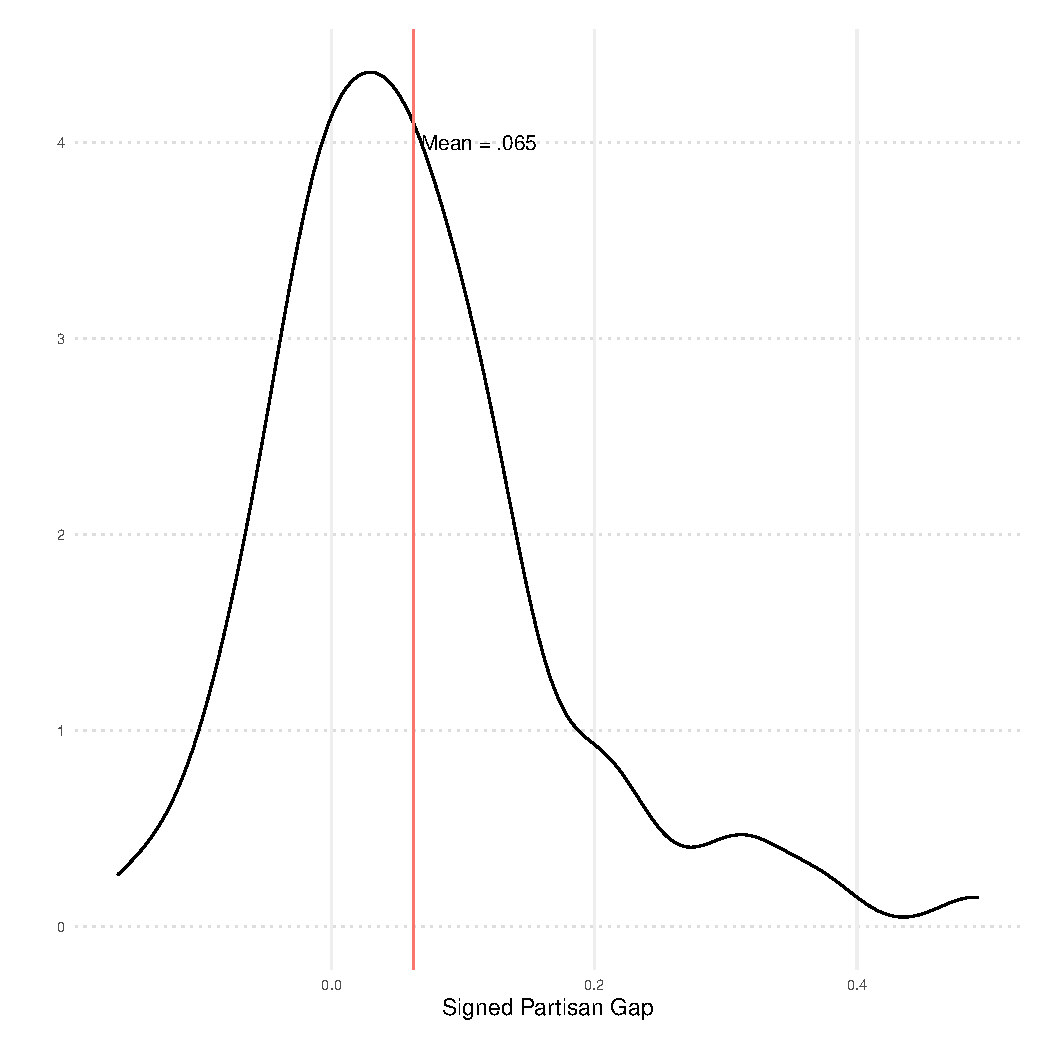
\includegraphics[scale=.8]{../figs/partisan_gap_density.pdf}
  \label{fig:figbias}
  \caption*{Kernel density plot. Positive gaps indicate instances in which partisans were \textit{more} accurate than their opponents about a party-congenial fact; negative gaps are those for which partisans were \textit{less} accurate than their opponents about a party-congenial fact. \textit{n}=187.}
\end{figure}
\end{center}

\vspace{-10mm}

Not only are the gaps relatively small on average, they are also not always consistently signed. Twenty eight percent (28\%) of these gaps are \textit{negative}; that is, on nearly three in ten knowledge items, partisans are less likely to know party-congenial facts than their opponents. Of the knowledge gaps in the expected direction, about half---45\%---are not statistically significant at the 95\% confidence level, despite an average sample size of 939 respondents per question. If we lower the threshold to the 90\% confidence level, 41\% of the positive gaps are not statistically distinguishable from zero. If we further limit our analysis to items with a sample size large enough to draw reliable conclusions (that is, when \textit{n}(Republicans) and \textit{n}(Democrats) both $\geq$ 100, or roughly 89\% of the items in our dataset), we find that 51\% of the positive gaps are not statistically significant at the 95\% confidence level.

Perhaps these findings are an artifact of our judgments regarding the expected sign of the partisan gap. While the vast majority of the items in our dataset have clear positive or negative implications for one party or another, for others, one might reasonably argue that the direction of the sign is debatable. For example, regarding a question about repayment of the 2009 financial bailout, one could argue that Republicans ``should'' know more on the topic as (1) the bailout was unpopular (thus signaling a negative connotation for Democrats) and (2) the GOP has traditionally made reducing government debt a central focus of its policy agenda. On the other hand, Democrats might be expected to be more correct in their answers because a high proportion (about 70\%) of the debt had been repaid in three years (a positive outcome under a Democratic president). In this case, the signed partisan gap could reasonably be coded as positive or negative. 

Importantly, our findings do not appear to be very sensitive to coding decisions. Averaging across the absolute value of all partisan gaps produces a mean gap of 9.2 percentage points, a median gap of 6.5 percentage points, and a standard deviation of 9.2 percentage points.\footnote{For the distribution of the absolute value of partisan gaps, please see \ref{fig:abs_part_gap}.} On a scale ranging from 0 to 100, these figures remain surprisingly small. 

\section*{Explaining Variation in Knowledge Gaps}

What explains variation in the size of partisan knowledge gaps? As is the case with other public opinion data, it is likely that question wording and response options influence how people respond to political knowledge questions. Here, we examine how such features might influence differences in the proportions of Democrats and Republicans who answer questions correctly.

To examine the degree to which these attributes affect the size of partisan gaps, we used an OLS model to predict the absolute value of partisan gaps as a function of survey and question characteristics. (We cluster our standard errors by survey to account for the fact that same people responded to multiple items.) As a starting point, we draw from \citet{luskinetal_nd}, which examines how question design features influence estimates of incorrect responding. Specifically, the authors show that the number of response options and phrasing of questions as a matter of opinion instead of fact can dramatically affect estimates of how much respondents know. Fewer response options, for example, may inflate the proportion of Democrats or Republicans who appear to know something, since fewer options increase the probability that a respondent will select the correct answer based on guessing alone \citep[][4]{luskinetal_nd}. Similarly, we might expect more of these ``false positives'' on close-ended questions compared to open-ended questions, since there is no opportunity to accidentally guess the right answer in the latter. Questions that provide ``don't know'' as a response option are less likely to have false positives, as they discourage guessing by providing an ``out'' to respondents. Of course, \citet{luskinetal_nd} examined how these features influence the \textit{levels} of misinformation in the \textit{population}, not differences between partisans, so it is plausible that these features affect the proportions of Democrats and Republicans who answer correctly in the same way. If, however, Democrats and Republicans differ in their propensity to guess the correct answer, we might expect the number and nature of response options to impact the size of knowledge gaps. To test this proposition, we coded both (a) the number of response options given by each question, and (b) whether the question offered an explicit ``don't know'' or ``not sure'' option (1) or not (0). We rescaled the former from 0-1 to aid in regression interpretation. 

We might also expect larger partisan knowledge gaps on questions that begin with phrases like ``do you think,'' ``do you believe,'' ``based on what you have heard,'' ``to the best of your knowledge,'' etc. These phrases likely encourage respondents who do not know the correct answer to choose what they see as the most probable response. In doing so, they are likely to rely upon what they would \textit{like} to believe the correct answer is, which would likely activate partisan reasoning and exacerbate observed differences in knowledge between Democrats and Republicans. Therefore, we coded questions that featured wording that encourages respondent guessing as 1, and 0 otherwise. 

In addition to the the features that \citet{luskinetal_nd} identify, there are several others that could also influence the size of partisan knowledge gaps. For example, answers to questions with a factually correct answer, by virtue of the phrasing of their response options, might ask respondents to make subjective \textit{assessments} instead of identify a concrete answer. Some questions---particularly those featured on the ANES----ask people to gauge whether the budget deficit increased, decreased, or remained about the same over a president's tenure, or how the rate of inflation changed over the past year. Because the response options for these questions are imprecise, people have a greater opportunity to interpret the meaning themselves \citep[e.g.][]{beyth_1982} using common heuristics, including partisanship \citep[e.g.][]{soodguess_2017}. As a result, a large partisan ``knowledge'' gap may reflect how partisans interpret response options rather than a true difference between what Democrats and Republicans know. Consider the case of two highly knowledgeable survey respondents (who perhaps work in the Bureau of Labor Statistics) who know definitively that the national unemployment rate in the United States grew from 4.0\% to 4.2\% over the past year, a time during which a Republican president occupied the White House. When the first respondent, a Democrat, is asked to evaluate how unemployment changed over the past year, she might (correctly) reason that unemployment ``got worse'' as the rate objectively increased over the previous 12 months. On the other hand, the second survey respondent, a Republican, might also (reasonably) conclude that 0.2 percentage points is a negligible change in unemployment, and might therefore be more liable to answer that the unemployment rate  ``stayed about the same'' over the past year. In this situation, two people who know \textit{the exact same fact} could plausibly choose two different response options and still be correct. The end result is that some ``knowledge gaps'' may be artificially large simply because respondents interpret the same response categories differently. For this reason, we add a dummy variable that captures whether or not a question featured vague response options, such as ``got better,'' ``stayed about the same,'' and ``got worse,'' in addition to ``definitely happened,'' ``probably happened,'' ''probably did not happen,'' and ``definitely did not happen.''

The mention of an elected official or party in a question is likely to exacerbate knowledge gaps, as these are likely to prime partisan thinking more than questions that do not reference political actors \citep[e.g.,][]{bisgaard_slothuus_2018,mondak_1993,Zaller1992}. We coded questions that reference a political actor (the president, or another prominent political figure) as 1 and questions that do not include a reference as 0 to determine whether source cues influence the knowledge differences between Democrats and Republicans.

We also include a dummy variable for any question that touches on a topic for which there exists a substantial amount of systematic misinformation. Although all of the questions included in our dataset have correct answers, several address topics about which significant portions of the population are ill-informed due to the proliferation of misinformation or conspiracy theories. These include, for example, questions related to global warming, Iraq's involvement in the 9/11 attacks, whether Iraq had weapons of mass destruction, whether Barack Obama is a Muslim, whether Obamacare autorized death panels, etc. Because belief in misinformation breaks down on distinctly partisan lines \citep{berinsky_2017,milleretal_2015,nyhan_2020}, we might expect larger than average knowledge gaps to emerge on these questions. We coded questions featuring topics tied to misinformation as 1 and 0 otherwise.\footnote{For a complete list of misinformation items, please see \ref{tab:misinfo_items}.}

Question difficulty likely plays a role in producing knowledge gaps. Specifically, questions that are more difficult to answer might incite larger partisan knowledge gaps, as Democrats and Republicans could rely on partisan heuristics to aid them in choosing a response. To gauge how question difficulty might influence knowledge gaps, we included a variable that documents the proportion of all respondents (not just Democrats or Republicans) who got the question correct. We reverse coded the variable so that higher question difficulty corresponds to a smaller proportion of respondents answering correctly, and rescaled it 0-1 to aid in interpretation. 

Of course, question wording features are likely not the sole determinants of differences in knowledge among Democrats and Republicans; the context in which surveys are administered may also influence variation in knowledge gaps. Surveys conducted during times in which politics is particularly salient---such as the fall of a presidential election year---may induce people to think about these knowledge questions in even more political (and therefore partisan) light. Just as Democrats and Republicans ``come home'' to their partisan leanings as Election Day approaches \citep{eriksonwlezien_2012,henderson_2015,sidesetal_2019,sidesvavreck_2013}, partisan bias may also increase as the campaign wears on, thus producing larger knowledge gaps on items included in surveys conducted closer to November in an election year. Accordingly, we include a dummy variable that takes a value of 1 if the survey in question was conducted in the fall of an election year (that is, conducted in September, October, or November) and 0 otherwise.

Additionally, we also include study fixed effects to determine whether any of the questions gathered in the context of different studies (that is, \citet{bullocketal_2015}, \citet{prior2015you}, \citet{jerit2012partisan}, or the ANES) produced larger partisan knowledge gaps than others. We omit questions featured on the ANES from the model to serve as a reference category. 


% Table created by stargazer v.5.2.2 by Marek Hlavac, Harvard University. E-mail: hlavac at fas.harvard.edu
% Date and time: Sat, Jan 01, 2022 - 9:20:27 PM
\begin{table}[!htbp] \centering 
  \caption{Predicting Absolute Value of the Partisan Gap} 
  \label{tab:tab1} 
\begin{tabular}{@{\extracolsep{5pt}}lc} 
\\[-1.8ex]\hline 
\hline \\[-1.8ex] 
 & \multicolumn{1}{c}{\textit{Dependent variable:}} \\ 
\cline{2-2} 
\\[-1.8ex] & Absolute Partisan Gap \\ 
\hline \\[-1.8ex] 
 Partisan Cue & $-$0.010 \\ 
  & (0.016) \\ 
  & \\ 
 Number of response options & $-$0.012$^{*}$ \\ 
  & (0.007) \\ 
  & \\ 
 Don't know/not sure & $-$0.032$^{**}$ \\ 
  & (0.014) \\ 
  & \\ 
 Encourages guessing & $-$0.014 \\ 
  & (0.015) \\ 
  & \\ 
 Response open to interpretation & 0.066$^{**}$ \\ 
  & (0.029) \\ 
  & \\ 
 Addresses misinformation & 0.067 \\ 
  & (0.060) \\ 
  & \\ 
 Question difficulty & $-$0.055 \\ 
  & (0.037) \\ 
  & \\ 
 Asked in fall of election year & $-$0.016 \\ 
  & (0.026) \\ 
  & \\ 
 Bullock et al. & 0.033 \\ 
  & (0.055) \\ 
  & \\ 
 Jerit and Barabas & $-$0.077 \\ 
  & (0.051) \\ 
  & \\ 
 Prior et al. & 0.029 \\ 
  & (0.061) \\ 
  & \\ 
 Constant & 0.174$^{***}$ \\ 
  & (0.058) \\ 
  & \\ 
\hline \\[-1.8ex] 
\hline 
\hline \\[-1.8ex] 
\textit{Note:}  & \multicolumn{1}{r}{$^{*}$p$<$0.1; $^{**}$p$<$0.05; $^{***}$p$<$0.01} \\ 
\end{tabular} 
\end{table} 


Table \ref{tab:tab1} shows the results of our analysis. Surprisingly, most features of question wording do not affect the size of partisan knowledge gaps. The effects of \textit{Partisan cue}, \textit{Number of response options}, \textit{Don't know/not sure}, \textit{Encourages guessing}, and \textit{Asked in fall of election year} are not statistically significant at conventional levels and are all of small substantive significance. Contrary to expectations, more difficult questions actually \textit{decrease} the size of the partisan gap. Perhaps more interestingly, we find a substantively significant effect related to whether a question features responses options that are open to interpretation. Those questions with vague response options like ``got better,'' ``stayed about the same,'' ``got worse,'' or featured ``probably'' or ``definitely'' increased partisan knowledge gaps by nearly six and a half percentage points compared to questions that did not ask respondents to make relative assessments. We also found the effect of \textit{Addresses misinformation} is rather large (about seven and a half percentage points) but very imprecisely estimated (\textit{se}=6.1\%).\footnote{We also analyzed variation by question topic, classifying questions into nine topic categories: those addressing with economic matters (e.g. inflation, unemployment, etc.), those related to foreign policy or national security, office/candidate recognition questions, those that address the environment, those that mention Social Security, those that refer to guns, those that touch on education, and a miscellaneous catch-all category (which includes, for example, questions related to marijuana, candidates' age, HIV/AIDS infection rates, etc.) The estimate for questions with responses open to interpretation increases to 7.3\%.} 

Interestingly, questions collected by \citet{jerit2012partisan} plausibly have somewhat smaller partisan knowledge gaps than those featured on the ANES (\textit{p}=0.231). This may be due to the fact that despite the authors' intent to gather questions with a ``partisan relevance,'' a sizable portion of questions in their dataset (roughly 27\%) do not have an immediate partisan implication. For example, it is unclear why a question asking about the proportion of teenagers who died from AIDS or another asking respondents to correctly identify the office held by Tommy Thompson (George W. Bush's Health and Human Services Secretary) should produce partisan knowledge gaps. Accordingly, we re-calculated the size of our partisan gap after removing questions (from all studies; about 21\%, remaining {n}=147) for which the partisan relevance was not clear. Doing so doesn't change the size of our mean partisan knowledge gap (6.7\%). 

\section*{Discussion and Conclusion}

Our results clarify our understanding of partisan knowledge gaps in important ways. First, partisan knowledge gaps are less ubiquitous than what conventional wisdom in political science suggests. For three in ten items, partisans either know \textit{less} party-congenial information or \textit{more} party-\textit{un}congenial information than their opponents. Among gaps occurring in the correct direction, we can only be certain that Democrats and Republicans actually differ from one another in their factual understanding of politics less than half the time. Secondly, the average knowledge gap in our data is small, with a mean gap of six percentage points and a median gap of about three percentage points. Third, many question features like the number of response options or question wording weakly predict the size of partisan knowledge gaps; instead, it is question difficulty and the \textit{content} of response options that influence the size of the gap.

If partisan gaps are small on average and difficult to predict based on question wording, why does the common wisdom that Democrats and Republicans differ substantially in political knowledge persist? One explanation may be that the knowledge items in our dataset are a not a representative set of relevant cognitions that partisans have. It may well be that the knowledge gaps are larger on partisan-relevant facts that are not asked about in the studies described above. To what degree this is so, we cannot say, except to note that the general bias is to ``hunt where the ducks are.'' That is, in at least two of our studies \citep{bullocketal_2015, prior2015you}, expert political scientists constructed knowledge questions that they reasonably believed \textit{a priori} would produce large partisan gaps; in the case of \citet{jerit2012partisan}, the authors built a dataset of knowledge questions that they believed carried a partisan implication (in other words, in which they expected knowledge gaps between Democrats and Republicans to occur). The fact that statistically significant, ``positive'' knowledge gaps only emerge on about half of the items from these studies suggests that partisan knowledge gaps are less common even when looking in the most obvious place. 

A potentially more satisfying explanation for this discrepancy is that such conventional wisdom is largely based on studies using data from the \citet{anes_gen}. Much of the literature on partisan knowledge gaps has built upon \citet{bartels_2002}, who was the first to write about these differences \citep{bullocklenz_2019}. For example, using the ANES data, \citet{bartels_2002} discovered that Democrats and Republicans reported different beliefs on a variety of objective facts---such as how inflation and unemployment changed over the previous eight years---while Ronald Reagan was president. In 1988, the estimated differences between Democrats and Republicans on knowledge questions ranged from approximately 12 to 36 percentage points, depending on the question.\footnote{These figures have been rescaled in percentage point terms. \citeapos{bartels_2002}  original calculation is that ``the estimated differences between Democrats and Republicans rang[e] from .249 to .715 on the -1 to +1 scales'' (137).} These kinds of questions with imprecise response options---which ask about respondents' \textit{assessment} of politically relevant facts rather than their actual \textit{knowledge} of such facts---are one of the most likely source of large partisan knowledge gaps. The fact that questions with imprecise response options are commonplace on one of the biggest publicly-available sources of survey data likely helps perpetuate the idea that Democrats and Republicans approach the political world with entirely different information. 

Based on our results here, we suspect that the vast majority of partisan gaps---when they do appear---are more likely to be a product of motivated responding than of partisans simply knowing different things (\citeauthor{bisgaard_slothuus_2018} \citeyear{bisgaard_slothuus_2018}; \citeauthor {bullocketal_2015} \citeyear{bullocketal_2015}; \citeauthor{prior2015you} \citeyear{prior2015you}; \citeauthor{schaffner_luks} \citeyear{schaffner_luks}; but see \citeauthor{berinsky_2017} \citeyear{berinsky_2017} and \citeauthor{peterson_iyengar_forth} \citeyear{peterson_iyengar_forth}). None of this is to say that partisan bias does not play a role in shaping how Democrats and Republicans interpret what they know; there is ample evidence to suggest that it does \citep[e.g.,][]{bisgaard2015bias, gainesetal_2007, khanna2018motivated}. Nor should the small size of the average gap prevent us from noting that on many of the questions, a majority of partisans on both sides of the aisle were either ignorant or misinformed about the facts: the average proportion of Republicans and Democrats who provided correct answers to these knowledge questions is about 42\% each. 

While this is certainly troubling for those who view political knowledge as an essential component of democratic citizenship, there is some reason for optimism. When it comes to knowledge of political facts, more often than not, there do not appear to be large imbalances between what Democrats and Republicans know. When partisan differences do emerge, we suspect that they are often more a product of biased interpretation of survey questions rather than of differential stores of knowledge. This suggests that even in a polarized political context, most Democrats and Republicans can use the same information to make collective judgments about whether to reward or punish elected officials based on performance---whether they want to, of course, is another question. 

\clearpage
\bibliographystyle{apsr}
\bibliography{pgap}

\clearpage

\appendix
\renewcommand{\thesection}{SI \arabic{section}}
\setcounter{table}{0}\renewcommand\thetable{\thesection.\arabic{table}}  
\setcounter{figure}{0}\renewcommand\thefigure{\thesection.\arabic{figure}}
\counterwithin{figure}{section}

\begin{center}
\Large \textbf{SUPPORTING INFORMATION}
\end{center}
\singlespacing
\vspace{-.4in}
\begin{center}
\section{Signed Partisan Gaps By Item}
\end{center}

% latex table generated in R 4.1.2 by xtable 1.8-4 package
% Sat Jan 01 21:20:27 2022
\begingroup\tiny
\begin{longtable}{lllcccccc}
\caption{Partisan Knowledge Gaps by Item} \\ 
  \hline
Item & Study & Year & R & n(R) & D & n(D) & Signed Gap & $\textit{p(Gap)}$ \\ 
  \hline
Unemployment over past year & ANES & 1986 & 0.366 &  276 & 0.301 &  532 & 0.065 & 0.060 \\ 
  Inflation over past year & ANES & 1986 & 0.431 &  276 & 0.427 &  532 & 0.004 & 0.903 \\ 
  Unemployment over past year & ANES & 1988 & 0.581 &  830 & 0.268 &  954 & 0.312 & 0.000 \\ 
  Inflation over past year & ANES & 1988 & 0.504 &  830 & 0.393 &  954 & 0.111 & 0.000 \\ 
  Deficit compared to 1980 & ANES & 1988 & 0.768 &  776 & 0.729 &  883 & -0.039 & 0.070 \\ 
  Social Security benefits since 1980 & ANES & 1988 & 0.490 &  774 & 0.393 &  900 & 0.096 & 0.000 \\ 
  School spending since 1980 & ANES & 1988 & 0.286 &  774 & 0.210 &  900 & 0.076 & 0.000 \\ 
  Unemployment over past year & ANES & 1992 & 0.684 &  928 & 0.885 & 1229 & 0.201 & 0.000 \\ 
  Inflation over past year & ANES & 1992 & 0.091 &  929 & 0.033 & 1229 & -0.057 & 0.000 \\ 
  Deficit under Clinton & ANES & 1996 & 0.247 &  654 & 0.341 &  894 & 0.094 & 0.000 \\ 
  Taxes under Clinton & ANES & 1996 & 0.599 &  652 & 0.373 &  896 & 0.226 & 0.000 \\ 
  Deficit compared to 1992 & ANES & 2000 & 0.513 &  646 & 0.606 &  821 & 0.094 & 0.000 \\ 
  Crime compared to 1992 & ANES & 2000 & 0.298 &  646 & 0.420 &  822 & 0.122 & 0.000 \\ 
  Unemployment over past year & ANES & 2004 & 0.442 &  446 & 0.109 &  518 & 0.334 & 0.000 \\ 
  Inflation over past year & ANES & 2004 & 0.376 &  445 & 0.603 &  518 & 0.227 & 0.000 \\ 
  Income tax for average person under Bush & ANES & 2004 & 0.298 &  485 & 0.131 &  592 & 0.167 & 0.000 \\ 
  Unemployment over past year & ANES & 2008 & 0.748 &  644 & 0.903 & 1343 & 0.155 & 0.000 \\ 
  Inflation over past year & ANES & 2008 & 0.189 &  646 & 0.148 & 1338 & 0.041 & 0.019 \\ 
  Unemployment over past year & ANES & 2012 & 0.092 & 1995 & 0.461 & 3102 & 0.369 & 0.000 \\ 
  Obama born in U.S. & ANES & 2012 & 0.200 & 1846 & 0.688 & 2888 & 0.488 & 0.000 \\ 
  Health care end of life & ANES & 2012 & 0.140 & 1843 & 0.378 & 2872 & 0.239 & 0.000 \\ 
  Government knew about 9/11 -2012 & ANES & 2012 & 0.239 & 1850 & 0.204 & 2889 & -0.036 & 0.003 \\ 
  Katrina flooding & ANES & 2012 & 0.519 & 1851 & 0.396 & 2883 & 0.123 & 0.000 \\ 
  Unemployment over past year & ANES & 2016 & 0.193 & 1728 & 0.559 & 1939 & 0.366 & 0.000 \\ 
  Existence of global warming & ANES & 2016 & 0.676 & 1723 & 0.904 & 1934 & 0.228 & 0.000 \\ 
  Cause of global warming & ANES & 2016 & 0.222 & 1724 & 0.530 & 1937 & 0.308 & 0.000 \\ 
  Government knew about 9/11 -2016 & ANES & 2016 & 0.261 & 1469 & 0.198 & 1665 & 0.063 & 0.000 \\ 
  Obama Muslim & ANES & 2016 & 0.501 & 1449 & 0.830 & 1661 & 0.329 & 0.000 \\ 
  Iraq casualties, 2007 vs. 2008 & Bullock et al. & 2008 & 0.756 &  123 & 0.476 &  143 & 0.281 & 0.000 \\ 
  Bush inflation change & Bullock et al. & 2008 & 0.533 &  122 & 0.857 &  140 & 0.324 & 0.000 \\ 
  Bush unemployment change & Bullock et al. & 2008 & 0.451 &  122 & 0.729 &  140 & 0.278 & 0.000 \\ 
  Estimated Bush approval & Bullock et al. & 2008 & 0.408 &  125 & 0.717 &  145 & 0.309 & 0.000 \\ 
  Iraq total casualties & Bullock et al. & 2008 & 0.756 &  123 & 0.631 &  141 & 0.125 & 0.029 \\ 
  Estimated Bush approval among Republicans & Bullock et al. & 2008 & 0.205 &  122 & 0.168 &  143 & 0.037 & 0.440 \\ 
  Obama age & Bullock et al. & 2008 & 0.573 &  124 & 0.662 &  142 & 0.089 & 0.135 \\ 
  McCain age & Bullock et al. & 2008 & 0.832 &  125 & 0.771 &  144 & 0.061 & 0.213 \\ 
  Afghanistan casualties, 2007 vs. 2008 & Bullock et al. & 2008 & 0.279 &  122 & 0.283 &  138 & 0.004 & 0.944 \\ 
  Bush deficit change & Bullock et al. & 2008 & 0.911 &  124 & 0.936 &  140 & 0.024 & 0.456 \\ 
  Defense spending & Bullock et al. & 2012 & 0.262 &   42 & 0.256 &   78 & 0.005 & 0.948 \\ 
  Iraq deaths & Bullock et al. & 2012 & 0.143 &   35 & 0.074 &   94 & -0.068 & 0.238 \\ 
  Iraq deaths: percent black & Bullock et al. & 2012 & 0.278 &   54 & 0.168 &   95 & 0.109 & 0.115 \\ 
  Bush II unemployment & Bullock et al. & 2012 & 0.093 &   43 & 0.088 &   91 & -0.005 & 0.924 \\ 
  Obama vote in 2008 & Bullock et al. & 2012 & 0.351 &   37 & 0.158 &   95 & 0.193 & 0.014 \\ 
  Global warming & Bullock et al. & 2012 & 0.377 &   53 & 0.444 &   81 & 0.067 & 0.445 \\ 
  Medicaid spending & Bullock et al. & 2012 & 0.105 &   38 & 0.299 &   97 & 0.194 & 0.018 \\ 
  Debt service spending & Bullock et al. & 2012 & 0.098 &   51 & 0.099 &   91 & 0.001 & 0.987 \\ 
  Obama unemployment & Bullock et al. & 2012 & 0.111 &   36 & 0.175 &   80 & -0.064 & 0.384 \\ 
  TARP: percent paid back & Bullock et al. & 2012 & 0.132 &   38 & 0.222 &   81 & 0.091 & 0.247 \\ 
  Foreign born population & Bullock et al. & 2012 & 0.264 &   53 & 0.395 &   86 & 0.131 & 0.116 \\ 
  Public debt & Prior et al. & 2008 & 0.155 &  181 & 0.153 &  215 & 0.001 & 0.974 \\ 
  Unemployment & Prior et al. & 2008 & 0.403 &  181 & 0.293 &  215 & 0.110 & 0.021 \\ 
  Uninsured & Prior et al. & 2008 & 0.475 &  181 & 0.270 &  215 & 0.205 & 0.000 \\ 
  Estate tax & Prior et al. & 2008 & 0.453 &  181 & 0.453 &  214 & -0.000 & 0.996 \\ 
  Gas price & Prior et al. & 2008 & 0.370 &  181 & 0.308 &  214 & -0.062 & 0.197 \\ 
  Unemployment & Prior et al. & 2004 & 0.432 &   88 & 0.233 &  146 & 0.199 & 0.001 \\ 
  Estate tax & Prior et al. & 2004 & 0.348 &   92 & 0.380 &  150 & 0.032 & 0.616 \\ 
  Debt & Prior et al. & 2004 & 0.239 &   92 & 0.216 &  148 & -0.023 & 0.681 \\ 
  Uninsured & Prior et al. & 2004 & 0.315 &   92 & 0.277 &  148 & 0.038 & 0.529 \\ 
  Poverty & Prior et al. & 2004 & 0.413 &   92 & 0.284 &  148 & 0.129 & 0.039 \\ 
  Talks with North Korea & Jerit \& Barabas & 2005 & 0.661 &  611 & 0.578 &  645 & 0.083 & 0.002 \\ 
  North Korea nuclear weapons - 2005 & Jerit \& Barabas & 2005 & 0.753 &  150 & 0.747 &  162 & 0.006 & 0.896 \\ 
  Iran nuclear weapons & Jerit \& Barabas & 2005 & 0.195 &  149 & 0.304 &  158 & -0.109 & 0.027 \\ 
  Patriot Act - hold terrorism suspects indefinitely & Jerit \& Barabas & 2004 & 0.211 &  161 & 0.303 &  142 & -0.092 & 0.068 \\ 
  Patriot Act - non-citizens before military tribunal & Jerit \& Barabas & 2004 & 0.323 &  161 & 0.275 &  142 & 0.048 & 0.361 \\ 
  Patriot Act - enter churches or attend rallies & Jerit \& Barabas & 2004 & 0.540 &  161 & 0.570 &  142 & -0.030 & 0.601 \\ 
  Iraq WMD - 2004 & Jerit \& Barabas & 2004 & 0.119 &  193 & 0.611 &  203 & 0.492 & 0.000 \\ 
  Iraq connected to 9/11 & Jerit \& Barabas & 2004 & 0.378 &  193 & 0.606 &  203 & 0.228 & 0.000 \\ 
  Saddam Hussein a threat to Middle East & Jerit \& Barabas & 2004 & 0.943 &  193 & 0.724 &  203 & 0.219 & 0.000 \\ 
  Saddam Hussein a threat to United States & Jerit \& Barabas & 2004 & 0.834 &  193 & 0.453 &  203 & 0.381 & 0.000 \\ 
  Iraq nuclear weapons & Jerit \& Barabas & 2003 & 0.739 &  375 & 0.576 &  335 & -0.163 & 0.000 \\ 
  North Korea nuclear weapons - 2003 & Jerit \& Barabas & 2003 & 0.432 &  375 & 0.454 &  335 & -0.022 & 0.561 \\ 
  North Korea chemical/biological weapons & Jerit \& Barabas & 2003 & 0.251 &  375 & 0.284 &  335 & -0.033 & 0.323 \\ 
  Office recognition - VP & Jerit \& Barabas & 2002 & 0.744 &  317 & 0.618 &  309 & 0.126 & 0.001 \\ 
  Office recognition - Secretary of State - 2002 & Jerit \& Barabas & 2002 & 0.607 &  298 & 0.504 &  345 & 0.103 & 0.009 \\ 
  Office recognition - Secretary of Defense & Jerit \& Barabas & 2002 & 0.390 &  326 & 0.308 &  315 & 0.082 & 0.030 \\ 
  Iran WMD & Jerit \& Barabas & 2002 & 0.468 &  361 & 0.431 &  299 & 0.037 & 0.346 \\ 
  North Korea WMD & Jerit \& Barabas & 2002 & 0.499 &  361 & 0.488 &  299 & 0.010 & 0.792 \\ 
  Issue behind Kyoto Protocol & Jerit \& Barabas & 2001 & 0.197 &  619 & 0.151 &  651 & 0.047 & 0.028 \\ 
  Senate approve tax cut & Jerit \& Barabas & 2001 & 0.591 &  171 & 0.433 &  210 & -0.157 & 0.002 \\ 
  Senate pass McCain-Feingold & Jerit \& Barabas & 2001 & 0.281 &  171 & 0.219 &  210 & -0.062 & 0.166 \\ 
  Limits on carbon emissions & Jerit \& Barabas & 2001 & 0.316 &  171 & 0.319 &  210 & -0.003 & 0.946 \\ 
  Regulation of arsenic in water & Jerit \& Barabas & 2001 & 0.222 &   54 & 0.302 &   63 & -0.079 & 0.336 \\ 
  Bush support of Kyoto Protocol & Jerit \& Barabas & 2001 & 0.226 &  164 & 0.222 &  212 & 0.004 & 0.928 \\ 
  Spending on education & Jerit \& Barabas & 2001 & 0.671 &  164 & 0.552 &  212 & -0.119 & 0.019 \\ 
  Regulations on lead & Jerit \& Barabas & 2001 & 0.207 &  164 & 0.175 &  212 & -0.033 & 0.422 \\ 
  Which candidate allows investment of SS in stocks/bonds & Jerit \& Barabas & 2000 & 0.372 &  624 & 0.286 &  756 & 0.086 & 0.001 \\ 
  Which candidate's wife advocates for mental illness & Jerit \& Barabas & 2000 & 0.426 &  624 & 0.470 &  756 & 0.043 & 0.108 \\ 
  Which candidate proposes missile defense system & Jerit \& Barabas & 2000 & 0.237 &  624 & 0.153 &  756 & 0.084 & 0.000 \\ 
  Which candidate proposes using surplus Medicaid \$ & Jerit \& Barabas & 2000 & 0.282 &  624 & 0.335 &  756 & 0.053 & 0.036 \\ 
  Next Democratic presidential nominee & Jerit \& Barabas & 2000 & 0.813 &  348 & 0.784 &  388 & -0.030 & 0.317 \\ 
  Next Republican presidential nominee & Jerit \& Barabas & 2000 & 0.856 &  348 & 0.786 &  388 & 0.070 & 0.013 \\ 
  Country stealing nuclear tech & Jerit \& Barabas & 1999 & 0.539 &  256 & 0.423 &  307 & 0.116 & 0.006 \\ 
  U.S. troops in Bosnia & Jerit \& Barabas & 1999 & 0.722 &  525 & 0.667 &  577 & 0.055 & 0.049 \\ 
  U.S. troops in Haiti & Jerit \& Barabas & 1999 & 0.383 &  525 & 0.300 &  577 & 0.083 & 0.004 \\ 
  Control of House - 1997 & Jerit \& Barabas & 1997 & 0.612 &  774 & 0.502 &  909 & 0.111 & 0.000 \\ 
  Gingrich ethics fine & Jerit \& Barabas & 1997 & 0.424 &  774 & 0.325 &  909 & -0.099 & 0.000 \\ 
  Trent Lott recognition & Jerit \& Barabas & 1997 & 0.262 &  183 & 0.133 &  203 & 0.129 & 0.001 \\ 
  Louis Freeh recognition & Jerit \& Barabas & 1997 & 0.120 &  183 & 0.079 &  203 & -0.041 & 0.174 \\ 
  John Huang recognition & Jerit \& Barabas & 1997 & 0.295 &  183 & 0.192 &  203 & 0.103 & 0.018 \\ 
  Kenneth Starr recognition & Jerit \& Barabas & 1997 & 0.311 &  183 & 0.167 &  203 & 0.144 & 0.001 \\ 
  Ralph Reed recognition & Jerit \& Barabas & 1997 & 0.142 &  183 & 0.118 &  187 & 0.024 & 0.486 \\ 
  Wester Hubbell recognition & Jerit \& Barabas & 1997 & 0.230 &  183 & 0.171 &  187 & 0.058 & 0.161 \\ 
  Office recognition - CT Dem Senator who lost primary & Jerit \& Barabas & 2006 & 0.498 &  241 & 0.448 &  221 & 0.050 & 0.284 \\ 
  Medicare drug plan - cost program for poor seniors & Jerit \& Barabas & 2006 & 0.364 &  733 & 0.331 &  834 & -0.033 & 0.167 \\ 
  Medicare drug plan - premium penalty & Jerit \& Barabas & 2006 & 0.591 &  733 & 0.588 &  834 & 0.003 & 0.898 \\ 
  Medicare drug plan - wait to switch & Jerit \& Barabas & 2006 & 0.414 &  186 & 0.432 &  220 & -0.018 & 0.718 \\ 
  Medicare drug plan - coverage gap & Jerit \& Barabas & 2006 & 0.312 &  186 & 0.327 &  220 & -0.015 & 0.740 \\ 
  Control of House - 2006 & Jerit \& Barabas & 2006 & 0.724 &  620 & 0.701 &  665 & 0.023 & 0.354 \\ 
  Office recognition - Secretary of State - 2006 & Jerit \& Barabas & 2006 & 0.497 &  620 & 0.469 &  665 & 0.028 & 0.323 \\ 
  Deadline for Medicare drug plan & Jerit \& Barabas & 2006 & 0.424 &  399 & 0.412 &  471 & 0.012 & 0.728 \\ 
  Financial penalty for no Rx coverage & Jerit \& Barabas & 2006 & 0.446 &  399 & 0.382 &  471 & 0.064 & 0.056 \\ 
  Blacks vs. whites better off - health insurance & Jerit \& Barabas & 2006 & 0.321 &  399 & 0.516 &  471 & 0.195 & 0.000 \\ 
  Blacks vs. whites better off - infant mortality & Jerit \& Barabas & 2006 & 0.273 &  399 & 0.418 &  471 & 0.145 & 0.000 \\ 
  Blacks vs. whites better off - life expectancy & Jerit \& Barabas & 2006 & 0.313 &  399 & 0.439 &  471 & 0.126 & 0.000 \\ 
  Latinos vs. whites better off - health insurance & Jerit \& Barabas & 2006 & 0.386 &  399 & 0.476 &  471 & 0.090 & 0.008 \\ 
  Latinos vs. whites better off - infant mortality & Jerit \& Barabas & 2006 & 0.391 &  399 & 0.359 &  471 & 0.032 & 0.329 \\ 
  Latinos vs. whites better off - life expectancy & Jerit \& Barabas & 2006 & 0.098 &  399 & 0.076 &  471 & 0.021 & 0.265 \\ 
  Blacks vs. whites - medical attention for heart disease & Jerit \& Barabas & 2006 & 0.358 &  399 & 0.499 &  471 & 0.141 & 0.000 \\ 
  Blacks vs. whites - medical attention for HIV/AIDS & Jerit \& Barabas & 2006 & 0.398 &  399 & 0.527 &  471 & 0.128 & 0.000 \\ 
  Clinton health plan - all Americans & Jerit \& Barabas & 1993 & 0.524 &  439 & 0.589 &  487 & 0.065 & 0.045 \\ 
  Clinton health plan - unemployed workers & Jerit \& Barabas & 1993 & 0.449 &  439 & 0.480 &  487 & 0.032 & 0.334 \\ 
  Congress considered - raise Medicare eligibility & Jerit \& Barabas & 1997 & 0.579 &  126 & 0.541 &  135 & 0.039 & 0.532 \\ 
  Congress considered - rich seniors pay higher Medicare premiums & Jerit \& Barabas & 1997 & 0.675 &  126 & 0.630 &  135 & 0.045 & 0.448 \\ 
  Congress considered - no Medicare for rich seniors & Jerit \& Barabas & 1997 & 0.341 &  126 & 0.385 &  135 & 0.044 & 0.463 \\ 
  Congress considered - expand choice under Medicare & Jerit \& Barabas & 1997 & 0.516 &  126 & 0.511 &  135 & -0.005 & 0.939 \\ 
  Congress considered - cut Medicare payments & Jerit \& Barabas & 1997 & 0.484 &  126 & 0.489 &  135 & -0.005 & 0.939 \\ 
  Existence of Medicare commission & Jerit \& Barabas & 1999 & 0.377 &  154 & 0.271 &  181 & -0.106 & 0.038 \\ 
  SOTU proposal - health care tax credits for elderly and disabled & Jerit \& Barabas & 1999 & 0.343 &  327 & 0.427 &  356 & 0.084 & 0.024 \\ 
  SOTU proposal - rich seniors pay more for Medicare & Jerit \& Barabas & 1999 & 0.260 &  327 & 0.247 &  356 & 0.013 & 0.702 \\ 
  SOTU proposal - use budget surplus for Medicare & Jerit \& Barabas & 1999 & 0.517 &  327 & 0.511 &  356 & -0.006 & 0.884 \\ 
  SOTU proposal - offer option to buy Medicaid before 65 & Jerit \& Barabas & 1999 & 0.239 &  327 & 0.225 &  356 & -0.014 & 0.669 \\ 
  SOTU proposal - use budget surplus for Social Security & Jerit \& Barabas & 1999 & 0.618 &  327 & 0.626 &  356 & 0.009 & 0.816 \\ 
  SOTU proposal - invest Social Security funds in stock market & Jerit \& Barabas & 1999 & 0.541 &  327 & 0.475 &  356 & -0.067 & 0.082 \\ 
  SOTU proposal - individual retirement savings accounts & Jerit \& Barabas & 1999 & 0.385 &  327 & 0.466 &  356 & -0.081 & 0.033 \\ 
  SOTU proposal - raising age for Social Security to 70 & Jerit \& Barabas & 1999 & 0.275 &  327 & 0.292 &  356 & 0.017 & 0.625 \\ 
  Pot panel rec - help cancer and AIDS pain & Jerit \& Barabas & 1999 & 0.545 &  341 & 0.551 &  361 & 0.006 & 0.878 \\ 
  Pot panel rec - no evidence of gateway drug & Jerit \& Barabas & 1999 & 0.226 &  341 & 0.277 &  361 & 0.051 & 0.119 \\ 
  Pot panel rec - pot smoke more toxic than tobacco smoke & Jerit \& Barabas & 1999 & 0.284 &  341 & 0.291 &  361 & 0.006 & 0.852 \\ 
  Medical error report - new government agency & Jerit \& Barabas & 1999 & 0.310 &  455 & 0.356 &  433 & 0.046 & 0.148 \\ 
  Medical error report - tougher malpractice laws & Jerit \& Barabas & 1999 & 0.233 &  455 & 0.189 &  433 & 0.044 & 0.112 \\ 
  SOTU proposal - offer option to buy Medicare before 65 & Jerit \& Barabas & 2000 & 0.344 &  256 & 0.451 &  346 & 0.107 & 0.008 \\ 
  SOTU proposal - rich seniors pay more for Medicare & Jerit \& Barabas & 2000 & 0.230 &  256 & 0.254 &  346 & -0.024 & 0.501 \\ 
  SOTU proposal - extend Medicare to provide Rx benefits & Jerit \& Barabas & 2000 & 0.477 &  256 & 0.624 &  346 & 0.148 & 0.000 \\ 
  SOTU proposal - expand CHIP to kids' parents & Jerit \& Barabas & 2000 & 0.359 &  256 & 0.442 &  346 & 0.083 & 0.041 \\ 
  SOTU proposal - tax credit for elderly health care & Jerit \& Barabas & 2000 & 0.250 &  256 & 0.402 &  346 & 0.152 & 0.000 \\ 
  Clinton SOTU health mention - children & Jerit \& Barabas & 1997 & 0.756 &   86 & 0.828 &  116 & 0.072 & 0.212 \\ 
  Clinton SOTU health mention - workers & Jerit \& Barabas & 1997 & 0.698 &   86 & 0.716 &  116 & 0.018 & 0.784 \\ 
  Clinton SOTU health mention - low-income people & Jerit \& Barabas & 1997 & 0.233 &   86 & 0.181 &  116 & 0.052 & 0.370 \\ 
  Clinton SOTU health mention - long-term care & Jerit \& Barabas & 1997 & 0.221 &   86 & 0.121 &  116 & 0.100 & 0.057 \\ 
  Budget agreement - increase senior premiums & Jerit \& Barabas & 1997 & 0.423 &  336 & 0.390 &  372 & 0.033 & 0.375 \\ 
  Budget agreement - prescription drugs & Jerit \& Barabas & 1997 & 0.315 &  336 & 0.331 &  372 & -0.015 & 0.667 \\ 
  Budget agreement - raising payroll tax & Jerit \& Barabas & 1997 & 0.295 &  336 & 0.242 &  372 & -0.053 & 0.114 \\ 
  Commission rec - increasing payroll taxes & Jerit \& Barabas & 1998 & 0.215 &  317 & 0.188 &  394 & -0.027 & 0.377 \\ 
  Commission rec - increasing retirement age & Jerit \& Barabas & 1998 & 0.669 &  317 & 0.596 &  394 & 0.072 & 0.047 \\ 
  Commission rec - investing Social Security \$ in stock market & Jerit \& Barabas & 1998 & 0.224 &  317 & 0.228 &  394 & 0.004 & 0.888 \\ 
  Commission rec - moving Social Security \$ to reitrement accounts & Jerit \& Barabas & 1998 & 0.445 &  317 & 0.302 &  394 & 0.143 & 0.000 \\ 
  Law to protect consumers in HMOs & Jerit \& Barabas & 1998 & 0.447 &  342 & 0.496 &  359 & -0.048 & 0.200 \\ 
  Right to sue HMO & Jerit \& Barabas & 1998 & 0.225 &  342 & 0.237 &  359 & -0.012 & 0.716 \\ 
  Senate gun bill - background checks at gun shows & Jerit \& Barabas & 1999 & 0.784 &  269 & 0.768 &  311 & -0.016 & 0.648 \\ 
  Senate gun bill - prohibits concealed carry & Jerit \& Barabas & 1999 & 0.405 &  269 & 0.347 &  311 & 0.058 & 0.151 \\ 
  Senate gun bill - raising gun owner age to 21 & Jerit \& Barabas & 1999 & 0.156 &  269 & 0.174 &  311 & -0.017 & 0.573 \\ 
  Senate gun bill - manufacture safety locks & Jerit \& Barabas & 1999 & 0.725 &  269 & 0.662 &  311 & -0.063 & 0.104 \\ 
  Senate gun bill - using gun illegal under 18 & Jerit \& Barabas & 1999 & 0.331 &  269 & 0.264 &  311 & 0.067 & 0.077 \\ 
  Clinton on guns - make agreement with NRA & Jerit \& Barabas & 2000 & 0.470 &  266 & 0.431 &  350 & -0.038 & 0.342 \\ 
  Clinton on guns - make agreement re: safety locks & Jerit \& Barabas & 2000 & 0.647 &  266 & 0.677 &  350 & 0.031 & 0.428 \\ 
  Clinton on guns - ask Congress to pass background checks & Jerit \& Barabas & 2000 & 0.699 &  266 & 0.726 &  350 & 0.026 & 0.472 \\ 
  Clinton on guns - discontinue gun buyback & Jerit \& Barabas & 2000 & 0.335 &  266 & 0.403 &  350 & 0.068 & 0.083 \\ 
  GWB on Social Security - reduce benefits & Jerit \& Barabas & 2000 & 0.484 &  314 & 0.347 &  398 & -0.137 & 0.000 \\ 
  GWB on Social Security - allow investment of SS payroll taxes & Jerit \& Barabas & 2000 & 0.494 &  314 & 0.382 &  398 & 0.112 & 0.003 \\ 
  GWB on Social Security - increase SS taxes & Jerit \& Barabas & 2000 & 0.468 &  314 & 0.281 &  398 & 0.187 & 0.000 \\ 
  Part of world with highest HIV/AIDS & Jerit \& Barabas & 2000 & 0.852 &  291 & 0.769 &  312 & -0.083 & 0.009 \\ 
  Teenagers die of AIDS & Jerit \& Barabas & 2000 & 0.399 &  291 & 0.449 &  312 & 0.050 & 0.214 \\ 
  Office recognition - Tommy Thompson & Jerit \& Barabas & 2001 & 0.302 &  305 & 0.223 &  337 & 0.079 & 0.023 \\ 
  Office recognition - John Ashcroft & Jerit \& Barabas & 2001 & 0.620 &  305 & 0.493 &  337 & 0.127 & 0.001 \\ 
  HIV infection rates & Jerit \& Barabas & 2002 & 0.418 &  388 & 0.463 &  341 & 0.046 & 0.214 \\ 
  HIV/AIDS prevention & Jerit \& Barabas & 2002 & 0.387 &  388 & 0.554 &  341 & 0.168 & 0.000 \\ 
  Spread of AIDS & Jerit \& Barabas & 2002 & 0.446 &  388 & 0.490 &  341 & 0.044 & 0.237 \\ 
  Medicare law - prescription drug benefit & Jerit \& Barabas & 2004 & 0.422 &  351 & 0.348 &  396 & -0.073 & 0.040 \\ 
  Medicare law - prescription drug discount card & Jerit \& Barabas & 2004 & 0.302 &  351 & 0.280 &  396 & -0.022 & 0.515 \\ 
  Medicare law - drug subsidy & Jerit \& Barabas & 2004 & 0.191 &  351 & 0.154 &  396 & -0.037 & 0.183 \\ 
  Medicare law - new cost estimates & Jerit \& Barabas & 2004 & 0.425 &  351 & 0.447 &  396 & 0.022 & 0.537 \\ 
  Discount card program - when available & Jerit \& Barabas & 2004 & 0.565 &  131 & 0.650 &  143 & 0.085 & 0.149 \\ 
  Discount card program - financial benefits for poor people & Jerit \& Barabas & 2004 & 0.382 &  131 & 0.364 &  143 & -0.018 & 0.759 \\ 
  Approval for military force in Iraq & Jerit \& Barabas & 2003 & 0.675 &  375 & 0.687 &  335 & -0.012 & 0.735 \\ 
  Iraq allow UN inspectors & Jerit \& Barabas & 2003 & 0.701 &  375 & 0.603 &  335 & 0.098 & 0.006 \\ 
  Public evidence about Iraq involvement in 9/11 & Jerit \& Barabas & 2003 & 0.659 &  375 & 0.597 &  335 & -0.062 & 0.090 \\ 
  Saddam Hussein threaten Israel & Jerit \& Barabas & 2003 & 0.453 &  375 & 0.487 &  335 & -0.033 & 0.376 \\ 
   \hline
\hline
\label{tab:indiv_items}
\end{longtable}
\endgroup


\clearpage

% latex table generated in R 4.1.2 by xtable 1.8-4 package
% Sat Jan 01 21:20:27 2022
\begin{table}[!htb]
\centering
\caption{Partisan Knowledge Gaps on Misinformation Items} 
\label{tab:misinfo_items}
\begingroup\tiny
\begin{tabular}{lllcccccc}
  \hline
Item & Study & Year & R & n(R) & D & n(D) & Signed Gap & $\textit{p(Gap)}$ \\ 
  \hline
Obama born in U.S. & ANES & 2012 & 0.200 & 1846 & 0.688 & 2888 & 0.488 & 0.000 \\ 
  Health care end of life & ANES & 2012 & 0.140 & 1843 & 0.378 & 2872 & 0.239 & 0.000 \\ 
  Government knew about 9/11 -2012 & ANES & 2012 & 0.239 & 1850 & 0.204 & 2889 & -0.036 & 0.003 \\ 
  Katrina flooding & ANES & 2012 & 0.519 & 1851 & 0.396 & 2883 & 0.123 & 0.000 \\ 
  Existence of global warming & ANES & 2016 & 0.676 & 1723 & 0.904 & 1934 & 0.228 & 0.000 \\ 
  Cause of global warming & ANES & 2016 & 0.222 & 1724 & 0.530 & 1937 & 0.308 & 0.000 \\ 
  Government knew about 9/11 -2016 & ANES & 2016 & 0.261 & 1469 & 0.198 & 1665 & 0.063 & 0.000 \\ 
  Obama Muslim & ANES & 2016 & 0.501 & 1449 & 0.830 & 1661 & 0.329 & 0.000 \\ 
  Global warming & Bullock et al. & 2012 & 0.377 &   53 & 0.444 &   81 & 0.067 & 0.445 \\ 
  Iraq WMD - 2004 & Jerit \& Barabas & 2004 & 0.119 &  193 & 0.611 &  203 & 0.492 & 0.000 \\ 
  Iraq connected to 9/11 & Jerit \& Barabas & 2004 & 0.378 &  193 & 0.606 &  203 & 0.228 & 0.000 \\ 
  Iraq nuclear weapons & Jerit \& Barabas & 2003 & 0.739 &  375 & 0.576 &  335 & -0.163 & 0.000 \\ 
  Public evidence about Iraq involvement in 9/11 & Jerit \& Barabas & 2003 & 0.659 &  375 & 0.597 &  335 & -0.062 & 0.090 \\ 
  Saddam Hussein threaten Israel & Jerit \& Barabas & 2003 & 0.453 &  375 & 0.487 &  335 & -0.033 & 0.376 \\ 
   \hline
\end{tabular}
\endgroup
\end{table}


\clearpage

\section{Knowledge Question Wordings and Correct Answers \label{si:q_text}}
\singlespacing

Correct answers are in bold unless otherwise noted. The correct answers to questions from the \citet{anes_gen} are based on information provided in the footnotes. The correct answers from \citet{bullocketal_2015}, \citet{jerit2012partisan}, and \citet{prior2015you} provided by the authors.\\

\vspace{.1in}

\large {\noindent{\textbf{\citet{anes_gen}}}}

\vspace{.2in}

\normalsize
   \begin{itemize}
\item \textbf{Unemployment over past year}\footnote{National unemployment rates based on information from the Bureau of Labor Statistics (available at \begin{footnotesize} \url{data.bls.gov} \end{footnotesize}). We followed the same coding scheme for unemployment data as described in \ref{append_q_text_anes_econ}.}  \\
Would you say that over the past year, the level of unemployment in the country has gotten better, stayed about the same, or gotten worse?\footnote{1986 version: ``Would you say that over the past year, the national unemployment rate has gotten better, stayed about the same, or gotten worse?''} 

\textit{Response options: Better, stayed about the same, gotten worse} 

         \begin{table}[H]
\centering
\caption{Unemployment over the past year - correct responses by year}
\vspace{.1in}
\label{unemp_corr_by_year}
\begin{tabular}{ll}
\textbf{Year} & \textbf{Correct answer}       \\
1986 & Stayed about the same                 \\
1988 & Better                 \\
1992 & Worse \\
2004 & Better \\
2008 & Worse \\
2012 & Better                 \\
2016 & Better \\
\end{tabular}
\end{table}
   \end{itemize}       

   \begin{itemize}
\item \textbf{Inflation over past year}\footnote{Inflation rates based on information from the Bureau of Labor Statistics (available at \begin{footnotesize} \url{data.bls.gov} \end{footnotesize}). The specific indicator is Consumer Price Index, All Urban Consumers, which according to BLS is the inflation index most reported by national media. To determine ``correct'' responses, we compared inflation levels from previous year's annual average. Inflation was considered to have stayed ``about the same'' if it did not increase or decrease more than one third of one percentage point from the previous year.} \\
Would you say that over the past year, inflation has gotten better, stayed about the same, or gotten worse?\footnote{1986 version: ``Would you say that over the past year, the inflation rate has gotten better, stayed about the same, or gotten worse?''} 

\textit{Response options: Better, stayed about the same, gotten worse}

         \begin{table}[H]
\centering
\caption{Inflation over the past year - correct responses by year}
\vspace{.1in}
\label{infl_corr_by_year}
\begin{tabular}{ll}
\textbf{Year} & \textbf{Correct answer}       \\
1986 & Stayed about the same                 \\
1988 & Stayed about the same                 \\
1992 & Better \\
2004 & Worse \\
2008 & Stayed about the same \\
\end{tabular}
\end{table}
   \end{itemize}   
   
  \begin{itemize}
\item \textbf{Gap between rich and poor - 2004, 2008, 2012, 2016}\footnote{Several sources, including \citet{Bartels2008} and \begin{footnotesize} \url{inequality.org} \end{footnotesize} demonstrate that the gap has been growing for decades.} \\
Do you think the difference in incomes between rich people and poor people in the United States today is larger, smaller, or about the same as it was 20 years ago?
\textit{Response options: \textbf{Larger}, smaller, stayed about the same}
\end{itemize}
 
\vspace{.2in}
\large \noindent\textit{1988}

\vspace{2mm}

\normalsize
\begin{itemize}
\item \textbf{Deficit compared to 1980}\footnote{Size of the federal budget deficit based on information from \begin{footnotesize} \url{usgovernmentspending.com} \end{footnotesize}, a site that aggregates federal data from multiple sources. Specific indicator used is Deficit-Federal in Billions of Nominal Dollars.}   \\
Would you say that compared to 1980 the federal budget deficit has gotten smaller, stayed about the same, or gotten larger? \\
\textit{Response options: Gotten smaller, stayed about the same, \textbf{gotten larger}} 
\end{itemize}

\begin{itemize}
\item \textbf{Social Security benefits since 1980}\footnote{Social Security benefits based on information from the Social Security Administration (\begin{footnotesize}\url{ssa.gov}\end{footnotesize}). The specific indicator is Minimum and Maximum Monthly Retired-Worker Benefits Payable to Individuals who Retired at age 62, 1957-2010 (Table A27).}   \\
Have Social Security benefits been increased, decreased, or stayed about the same as they were in 1980, or haven't you paid much attention to this? \\
\textit{Response options: \textbf{Increased}, decreased, stayed about the same} 
\end{itemize}

\begin{itemize}
\item \textbf{School spending since 1980}\footnote{School spending based on information from the Department of Education \begin{footnotesize}\url{ed.gov}\end{footnotesize}. Specific indicator used is Total Spending, Elementary and Secondary - Appropriation Numbers.}   \\
Has federal spending on public schools been increased, decreased, or stayed about the same as it was in 1980, or haven't you paid much attention to this? \\
\textit{Response options: Increased, \textbf{decreased}, stayed about the same} 
\end{itemize}

\vspace{2mm}

\large \noindent\textit{1996}

\vspace{2mm}

\normalsize
\begin{itemize}
\item \textbf{Deficit under Clinton}\footnote{Deficit based on information from \begin{footnotesize}\url{usgovernmentspending.com}\end{footnotesize}, a site that aggregates federal data from multiple sources. Specific indicator used is Federal Deficit in Nominal Billions of Dollars.} \\
Would you say that the size of the yearly budget deficit increased, decreased, or stayed about the same during Clinton's time as President?         \\     
\textit{Response options: \textbf{Increased}, decreased, stayed about the same} 
\end{itemize}

\normalsize
\begin{itemize}
\item \textbf{Taxes under Clinton}\footnote{Tax rates based on information contained in \citet{allen_1996}.} \\
Would you say that the federal income tax paid by the average working person has increased, decreased, or stayed about the same during Clinton's time as President?      \\
\textit{Response options: \textbf{Increased}, decreased, stayed about the same} 
\end{itemize}

\vspace{2mm}

\large \noindent\textit{2000}

\vspace{2mm}

\normalsize
\begin{itemize}
\item \textbf{Deficit compared to 1992}\footnote{Size of the federal budget deficit based on information from \begin{footnotesize}\url{usgovernmentspending.com}\end{footnotesize}, a site that aggregates federal data from multiple sources. Specific indicator used is Deficit-Federal in Billions of Nominal Dollars.} \\
As you know, Bill Clinton was first elected President in November 1992. He will soon be leaving office after 8 years as President. The next several questions ask whether you think things have changed since Clinton came into office. First, would you say that compared to 1992, the federal budget deficit is now smaller, larger, or about the same?        \\     
\textit{Response options: Gotten smaller, \textbf{gotten larger}, about the same} \\
\end{itemize}

\normalsize
\begin{itemize}
\item \textbf{Crime rate compared to 1992}\footnote{Crime rate based on information from the Brennan Center (available at \begin{footnotesize}\url{https://www.brennancenter.org/sites/default/files/publications/Crime\%20Trends\%201990-2016.pdf}\end{footnotesize}).} \\
Would you say that compared to 1992 the nation's crime rate has gotten better, gotten worse, or stayed about the same?        \\     
\textit{Response options: \textbf{Better}, worse, the same} \\
\end{itemize}

\large \noindent\textit{2004}

\normalsize
\begin{itemize}
\item \textbf{Income tax for average person under Bush}\footnote{Income tax information based on information from the Center on Budget and Policy Priorities (available at \begin{footnotesize}\url{https://www.cbpp.org/sites/default/files/atoms/files/3-31-17tax.pdf}\end{footnotesize}).} \\
Would you say that, compared to 2000, the federal income tax paid by the average working person has increased, decreased, or stayed about the same during George W. Bush's time as President?        \\     
\textit{Response options: Increased, \textbf{decreased}, stayed about the same} \\
\end{itemize}


\large \noindent\textit{2012}

\normalsize
\begin{itemize}
\item \textbf{Obama born in U.S.} \\
Was Barack Obama definitely born in the United States, probably born in the United States, probably born in another country, or definitely born in another country?  \\     
\textit{Response options: \textbf{Definitely born in the U.S.}, probably born in the U.S., probably born in another country, definitely born in another country} \\
\end{itemize}

\normalsize
\begin{itemize}
\item \textbf{Health care end of life} \\
Does the health care law passed in 2010 definitely authorize government panels to make end-of-life decisions for people on Medicare, probably authorize government panels to make end-of-life decisions for people on Medicare, probably not authorize government panels to make end-of-life decisions for people on Medicare, or definitely not authorize government panels to make end-of-life decisions for people on Medicare?  \\     
\textit{Response options: Definitely authorizes, probably authorizes, probably does not authorize, \textbf{definitely does not authorize}} \\
\end{itemize}

\normalsize
\begin{itemize}
\item \textbf{Government knew about 9/11 - 2012} \\
Did senior federal government officials definitely know about the terrorist attacks on September 11, 2001 before they happened, probably knew about the terrorist attacks on September 11, 2001 before they happened, probably did not know about the terrorist attacks on September 11, 2001 before they happened, or definitely did not know about the terrorist attacks on September 11, 2001 before they happened?  \\     
\textit{Response options: Definitely knew, probably knew, probably did not know, \textbf{definitely did not know}} \\
\end{itemize}

\normalsize
\begin{itemize}
\item \textbf{Katrina flooding} \\
Some people say that when Hurricane Katrina hit the Gulf Coast in the summer of 2004, the federal government intentionally breached flood levees in New Orleans so that poor neighborhoods would be flooded and middle-class neighborhoods would be spared. Do you think the federal government definitely did this, probably did this, probably did not do this, or definitely did not do this?  \\     
\textit{Response options: Definitely did this, probably did this, probably did not do this, \textbf{definitely did not do this}} \\
\end{itemize}

\large \noindent\textit{2016}

\normalsize
\begin{itemize}
\item \textbf{Global warming happening}\footnote{Information on global warming taken from the Union of Concerned Scientists (available at \begin{footnotesize}\url{https://www.ucsusa.org/global-warming}\end{footnotesize}).} \\
You may have heard about the idea that the world's temperature may have been going up slowly over the past 100 years. What is your personal opinion on this? Do you think this has probably been happening, or do you think it probably hasn't been happening?      \\     
\textit{Response options: \textbf{Has probably been happening}, probably hasn't been happening} \\
\end{itemize}

\normalsize
\begin{itemize}
\item \textbf{Global warming cause}\footnote{Information on global warming taken from the Union of Concerned Scientists (available at \begin{footnotesize}\url{https://www.ucsusa.org/global-warming}\end{footnotesize}).} \\
(Do/Assuming it's happening, do) you think a rise in the world's temperatures would be caused mostly by human activity, mostly by natural causes, or about equally by human activity and by natural causes?  \\     
\textit{Response options: \textbf{Mostly by human activity}, mostly by natural causes, about equally by human activity and natural causes} \\
\end{itemize}

\normalsize
\begin{itemize}
\item \textbf{Government knew about 9/11 - 2016} \\
Did senior federal government officials definitely know about the terrorist attacks on September 11, 2001 before they happened, probably knew about the terrorist attacks on September 11, 2001 before they happened, probably did not know about the terrorist attacks on September 11, 2001 before they happened, or definitely did not know about the terrorist attacks on September 11, 2001 before they happened?  \\     
\textit{Response options: Definitely knew, probably knew, probably did not know, \textbf{definitely did not know}}\footnote{The order of response options was randomized.} \\
\end{itemize}

\normalsize
\begin{itemize}
\item \textbf{Obama Muslim} \\
Is Barack Obama a Muslim, or is he not a Muslim?  \\     
\textit{Response options: Muslim, \textbf{Not a Muslim}} \\
\end{itemize}





\large {\noindent{\textbf{\citet{bullocketal_2015}}}}

\vspace{.2in}

\noindent{\textit{2008 CCES Study}}

\normalsize 
   \begin{itemize}
       \item \textbf{Iraq casualties, 2007 vs. 2008} \\
       Was the number of U.S. soldiers killed in Iraq in the first half of 2008 lower, about the same, or higher than the number who were killed in the second half of 2007?
       \\\textit{Response options: \textbf{lower (0)}, about the same (.5), higher (1)}
   \end{itemize}
   
      \begin{itemize}
       \item \textbf{Bush inflation change} \\
       Compared to January 2001, when President Bush first took office, has the level of inflation in the country increased, stayed the same, or decreased?
 \\\textit{Response options: \textbf{increased}, stayed about the same, decreased}
   \end{itemize}

     \begin{itemize}
       \item \textbf{Bush unemployment change} \\
       Compared to January 2001, when President Bush first took office, has the level of unemployment in the country increased, stayed the same, or decreased?
 \\\textit{Response options: \textbf{increased}, stayed about the same, decreased}
   \end{itemize}
   
        \begin{itemize}
       \item \textbf{Estimated Bush approval} \\
       About what percentage of \textit{Americans} approve of the way that George W. Bush is handling his job as President?
\\ \textit{Response options: \textbf{20\%}, 30\%, 40\%, 60\%, 60\%}
   \end{itemize}
   
\begin{itemize}
\item \textbf{Iraq total casualties} \\
  About how many U.S. soldiers have been killed in Iraq since the invasion in March 2003?
\\ \textit{Response options: \textbf{4,000}, 8,000, 12,000, 16,000, 20,000}
   \end{itemize}

\begin{itemize}
\item \textbf{Estimated Bush approval among Republicans} \\
  About what percentage of \textit{Republicans} approve of the way George W. Bush is handling his job as president?
\\ \textit{Response options: 40\%, 50\%, \textbf{60\%}, 70\%, 80\%}
   \end{itemize}
   
   \begin{itemize}
\item \textbf{Obama age} \\
  How old is Barack Obama?
\\ \textit{Response options: 37, 42, \textbf{47}, 52}
   \end{itemize}

   \begin{itemize}
\item \textbf{McCain age} \\
  How old is John McCain?
\\ \textit{Response options: 62, 67, \textbf{72}, 77}
   \end{itemize}


\begin{itemize}
\item \textbf{Afghanistan casualties, 2007 vs. 2008} \\
  Was the number of U.S. soldiers killed in Afghanistan in the first half of 2008 lower, about the same, or higher than the number who were killed in the second half of 2007?

 \textit{Response options: lower, \textbf{about the same}, higher}
   \end{itemize}

\begin{itemize}
\item \textbf{Bush deficit change} \\
Compared to January 2001, when President Bush first took office, has the federal budget deficit in the country increased, stayed the same, or decreased?

\textit{Response options: \textbf{increased}, stayed about the same, decreased}
   \end{itemize}

\large \noindent{\textit{2012 MTurk Study}}

\normalsize 

\begin{itemize}
\item \textbf{Defense spending} \\
For every dollar the federal government spent in fiscal year 2011, about how much went to the Department of Defense (US Military)?
\\ \textit{Range of response line: 3 to 27 cents}
\\ \textit{Correct response: \textbf{19.4 cents}}
   \end{itemize}

\begin{itemize}
\item \textbf{Iraq deaths} \\
About how many U.S. soldiers were killed in Iraq between the invasion in 2003 and the withdrawal of troops in December 2011?
 \textit{Range of response line: 1,000 to 7,000}
\\ \textit{Correct response: \textbf{4,486}}
   \end{itemize}

\begin{itemize}
\item \textbf{Iraq deaths: percent black} \\
Approximately 12 to 13\% of the US population is Black. What percentage of US Soldiers killed in Iraq since the invasion in 2003 are Black?

 \textit{Range of response line: 9\% to 21\%}
\\ \textit{Correct response: \textbf{9.90\%}}
   \end{itemize}

\begin{itemize}
\item \textbf{Bush II unemployment} \\
From January 2001, when President Bush first took office, to January 2009, when President Bush left office, how had the unemployment rate in the country changed?
\\ \textit{Range of response line: -2\% (unemployment decreased) to 4\% (unemployment increased)}
\\ \textit{Correct response: \textbf{increased by 3.6\%}}
   \end{itemize}

\begin{itemize}
\item \textbf{Obama vote in 2008} \\
In the 2008 Presidential Election, Barack Obama defeated his Republican challenger John McCain. In the nation as a whole, of all the votes cast for Obama and McCain, what percentage went to Obama?

 \textit{Range of response line: 50\% to 62\%}
\\ \textit{Correct response: \textbf{53.70\%}}
   \end{itemize}
   
   \begin{itemize}
\item \textbf{Global warming} \\
According to NASA, by how much did annual average global temperatures, in degrees Fahrenheit, differ in 2010 from the average annual global temperature between 1951 and 1980?
 \textit{Range of response line: -1 (temperatures cooler) to 2 (temperatures warmer)}
\\ \textit{Correct response: \textbf{increased by 1.1 degrees}}
   \end{itemize}

\begin{itemize}
\item \textbf{Medicaid spending} \\
Medicaid is a jointly funded, Federal-State health insurance program for low-income and needy people. For every dollar the federal government spent in fiscal year 2011, about how much went to Medicaid?

 \textit{Range of response line: 3 to 27 cents}
\\ \textit{Correct response: \textbf{7.5 cents}}
   \end{itemize}

\begin{itemize}
\item \textbf{Debt service spending} \\
The Treasury Department finances U.S. Government debt by selling bonds and other financial products. For every dollar the federal government spent in fiscal year 2011, about how much went to pay interest on those Treasury securities?

 \textit{Range of response line: 3 to 27 cents}
\\ \textit{Correct response: \textbf{6.2 cents}}
   \end{itemize}

\begin{itemize}
\item \textbf{Obama unemployment} \\
From January 2009, when President Obama first took office, to February 2012, how had the unemployment rate in the country changed?
\\ \textit{Range of response line: -2\% (unemployment decreased) to 4\% (unemployment increased)}
\\ \textit{Correct response: \textbf{increased by 0.5\%}}
   \end{itemize}

\begin{itemize}
\item \textbf{TARP: percent paid back} \\
The Treasury Department initiated TARP (the first bailout) during the financial crisis of 2008. TARP involved loans to banks, insurance companies, and auto companies. Of the \$414 billion spent, what percentage had been repaid, as of March 15, 2012?
 \textit{Range of response line: 1 (less repaid) to 100 (more repaid)}
\\ \textit{Correct response: \textbf{69.56\%}}
   \end{itemize}

\begin{itemize}
\item \textbf{Foreign born population} \\
According to the Census Bureau, in 2010 what percentage of the total population of the United States was born outside of the United States (foreign-born)?

 \textit{Range of response line: 1 to 100\%}
\\ \textit{Correct response: \textbf{12.92\%}}
   \end{itemize}

\vspace{.2in}

\large {\noindent{\textbf{\citet{prior2015you}}}}

\vspace{.2in}

\noindent{\textit{2004 Study}}
\normalsize
\begin{itemize}
\item \textbf{Unemployment} \\
The U.S. Bureau of Labor Statistics counts a person as unemployed if they are not employed at any job and are looking for work. By this definition, what percentage of Americans was unemployed in August of 2004? If you do not know the answer, please give us your best guess.

 \textit{Response options: around 11\%, around 9\%, around 7\%, \textbf{around 5\%}, around 3\%}
   \end{itemize}

\begin{itemize}
\item \textbf{Estate tax} \\
There is a federal estate tax---that is, a tax on the money people leave to others when they die. What percentage of Americans leaves enough money to others for the federal estate tax to kick in? If you do not know the answer, please give us your best guess.

 \textit{Response options: about 95\% of all Americans, about 70\% of all Americans, about 50\% of all Americans, about 25\% of all Americans, \textbf{less than 5\% of Americans}}
   \end{itemize}

\begin{itemize}
\item \textbf{Debt} \\
The outstanding public debt of the United States is the total amount of money owed by the federal government. Every year the government runs a deficit, the size of the public debt grows. Every year the government runs a surplus, the size of the public debt shrinks. In January of 2001, when President Bush took office, the outstanding public debt of the United States was approximately 5.7 trillion dollars. Which of the following responses is closest to the outstanding public debt today? If you do not know the answer, please give us your best guess.

 \textit{Response options: less than 3.5 trillion dollars, 4.5 trillion dollars, 5.5 trillion dollars, 6.5 trillion dollars, \textbf{7.5 trillion dollars}, 8.5 trillion dollars, more than 9.5 trillion dollars}
   \end{itemize}

\begin{itemize}
\item \textbf{Uninsured} \\
In August 2004, the United States Census Bureau reported an estimate of the number of Americans without health insurance. The Census Bureau classified people as uninsured if they were not covered by any type of health insurance at any time in 2003. By this definition, what percentage of Americans did not have health insurance in 2003? If you do not know the answer, please give us your best guess.

\textit{Response range: 0-100\%} \\
\textit{Correct response: \textbf{12.6-18.6\%}}
   \end{itemize}

\begin{itemize}
\item \textbf{Poverty} \\
In August 2004, the Census Bureau reported how many Americans live in poverty. The poverty threshold depends on the size of the household. For example, a person under age 65 is considered to live in poverty if his or her 2003 income was below \$9,573 and a family of four is considered to live in poverty if its 2003 income was below \$18,810. By this definition, what percentage of Americans lived in poverty in 2003? If you do not know the answer, please give us your best guess.

\textit{Response range: 0-100\%} \\
\textit{Correct response: \textbf{9.5-15.5\%}}
   \end{itemize}

   \large \noindent{\textit{2008 Study}}

\normalsize
\begin{itemize}
\item \textbf{Unemployment} \\
The U.S. Bureau of Labor Statistics counts a person as unemployed if the person is not employed at any job and is looking for work. By this definition, 4.7 percent of Americans were unemployed in 2001 [at the beginning of President Bush's first term in office]. What percentage of Americans are currently unemployed?

\textit{Response range: 0-100\%} \\
\textit{Correct response: \textbf{4.2-5.4\%}} 
   \end{itemize}
   
\begin{itemize}
\item \textbf{Estate tax} \\
There is a federal estate tax---that is, a tax on the money people leave to others when they die. [President Bush has repeatedly proposed to eliminate the estate tax.] What percentage of Americans leave enough money to others for the federal estate tax to kick in?

\textit{Response options: \textbf{less than 5\% of all Americans}, about 25\% of all Americans, about 50\% of all Americans, about 75\% of all Americans, about 95\% of all Americans}
   \end{itemize}
   
   \begin{itemize}
\item \textbf{Debt} \\
The outstanding public debt of the United States is the total amount of money owed by the federal government. Every year the government runs a deficit, the size of the public debt grows. Every year the government runs a surplus, the size of the public debt shrinks. [In January of 2001, when President Bush took office, the outstanding public debt of the United States was approximately 5.7 trillion dollars.] Which of the following responses is closest to the outstanding public debt today? 

\textit{Response options: less than 5.5 trillion dollars, 6.5 trillion dollars, 7.5 trillion dollars, 8.5 trillion dollars, \textbf{9.5 trillion dollars}, 10.5 trillion dollars, more than 11.5 trillion dollars}
   \end{itemize}
 
   \begin{itemize}
\item \textbf{Uninsured} \\
Each year, the United States Census Bureau reports an estimate of the number of Americans without health insurance. The Census Bureau classifies people as uninsured if they were not covered by any type of health insurance at any time during the year. By this definition, 14.1 percent of Americans did not have health insurance in 2001[, the year President Bush took office]. According to the latest estimate (for 2006), what percentage of Americans do not have health insurance? 

\textit{Response range: 0-100\%} \\
\textit{Correct response: \textbf{12.6-19.0\%}} 
   \end{itemize}

   \begin{itemize}
\item \textbf{Gas price} \\
According to the American Automobile Association (AAA), the national average price for a gallon of regular gasoline was \$1.49 [at the beginning of George W. Bush's presidency] in January 2001. What is the current national average price for a gallon of regular gasoline?

\textit{Response range: open-ended; format given \$xx.xx} \\
\textit{Correct response: \textbf{3.22-3.32}} 
   \end{itemize}
   
   \vspace{.2in}
   

\large {\noindent{\textbf{\citet{jerit2012partisan}}}}
\vspace{.1in} \\
\normalsize

\noindent \citet{jerit2012partisan} sourced questions from multiple surveys in their study. We present them in chronological order below. Correct responses provided by the authors unless otherwise noted. 

\vspace{.2in}

 \large \noindent \textit{1993}
\normalsize
   \begin{itemize}
\item \textbf{Clinton health plan - all Americans} \\
Do you happen to know, does the (President Bill) Clinton health care reform plan guarantee health insurance coverage to all Americans, or doesn't the plan go that far? 

\textit{Response options: \textbf{Yes, guarantees}; no; does not guarantee} 
\end{itemize}

\begin{itemize}
\item \textbf{Clinton health plan - unemployed workers} \\
Do you happen to know, does the (President Bill) Clinton health care reform plan guarantee health insurance coverage to all Americans, or doesn't the plan go that far? 

\textit{Response options: \textbf{Yes, guarantees}; no; does not guarantee} 
\end{itemize}
  

 \large \noindent \textit{1997} 
\normalsize
\begin{itemize} \item{[Common introduction] As I read each of the following, please tell me to the best of your knowledge if Congress considered proposals to...

   \begin{itemize}
\item \textbf{Congress considered - raise Medicare eligibility} \\
...Gradually raise the age at which someone is eligible for Medicare from 65 to 67...or not?

\textit{Response options: \textbf{Yes}; no} 
\end{itemize}

   \begin{itemize}
\item \textbf{Congress considered - rich seniors pay higher Medicare premiums} \\
...Require upper income seniors to pay higher Medicare premiums...or not?

\textit{Response options: \textbf{Yes}; no} 
\end{itemize}

   \begin{itemize}
\item \textbf{Congress considered - no Medicare for rich seniors} \\
...No longer provide Medicare to upper income seniors who can afford other health insurance...or not?

\textit{Response options: Yes; \textbf{no}} 
\end{itemize}

   \begin{itemize}
\item \textbf{Congress considered - expand choice under Medicare} \\
....Give seniors wider choice of health plans under Medicare…or not?

\textit{Response options: \textbf{Yes}; no} 
\end{itemize}

   \begin{itemize}
\item \textbf{Congress considered - cut Medicare payments} \\
...Cut Medicare payments to doctors, hospitals, and HMOs...or not?

\textit{Response options: \textbf{Yes}; no} 
\end{itemize}}
\end{itemize}

\begin{itemize}
\item{[Common introduction] (I would like to ask you a few questions about some things that have been in the news recently. Not everyone will have heard about them.)... In his (State of the Union) speech (January, 1997), did (Bill) Clinton propose expanding health care coverage to...

   \begin{itemize}
\item \textbf{Clinton SOTU health mention - children} \\
...Children?

\textit{Response options: \textbf{Yes}; no} 
\end{itemize}

   \begin{itemize}
\item \textbf{Clinton SOTU health mention - workers} \\
...Working people who are currently uninsured?

\textit{Response options: \textbf{Yes}; no}
\end{itemize}

   \begin{itemize}
\item \textbf{Clinton SOTU health mention - low-income people} \\
...All low-income people?

\textit{Response options: Yes; \textbf{no}} 
\end{itemize}

   \begin{itemize}
\item \textbf{Clinton SOTU health mention - long-term care} \\
...People who need long term care?

\textit{Response options: Yes; \textbf{no}} 
\end{itemize}}
\end{itemize}

\begin{itemize}
\item {[Common introduction] (I would like to ask you a few questions about some things that have been in the news recently. Not everyone will have heard of them.) As you may know, the budget agreement by President Bill Clinton and members of Congress to balance the budget by the year 2002 included many specific measures having to do with Medicare. As far as you know, does the plan call for...

   \begin{itemize}
\item \textbf{Budget agreement - increase senior premiums} \\
...Increasing premiums for all elderly Americans, or not?

\textit{Response options: \textbf{Yes, part of plan}; no, not part of plan} 
\end{itemize}

   \begin{itemize}
\item \textbf{Budget agreement - prescription drugs} \\
...Adding a new prescription drug benefit, or not?

\textit{Response options: Yes, part of plan; \textbf{no, not part of plan}} 
\end{itemize}

   \begin{itemize}
\item \textbf{Budget agreement - raising payroll tax} \\
...Raising the payroll tax that pays for part of Medicare?

\textit{Response options: Yes, part of plan; \textbf{no, not part of plan}} 
\end{itemize}}
\end{itemize}

   \begin{itemize}
\item \textbf{Control of House - 1997} \\
Do you happen to know which political party has a majority in the U.S. House of Representatives?

\textit{Response options: \textbf{Republicans}; Democrats} 
\end{itemize}

   \begin{itemize}
\item \textbf{Gingrich ethics fine} \\
Do you happen to know who lent New Gingrich the money he needed to pay off his ethics fine?

\textit{Response options: open-ended} \\
\textit{Correct answer: \textbf{Bob Dole}} 
\end{itemize}

\begin{itemize}
\item {[Common introduction] I'm going to read a list of names of people who have been in the news. Not everyone will have heard of them. For each one, please tell me if you happen to know who that person is. 

   \begin{itemize}
\item \textbf{Trent Lott recognition} \\
Trent Lott (If yes, ask:) Who is Trent Lott?

\textit{Response options: Open-ended} \\
\textit{Correct response: \textbf{coded by Pew [Senate Majority Leader]}}
\end{itemize}

   \begin{itemize}
\item \textbf{Louis Freeh recognition} \\
Louis Freeh (If yes, ask:) Who is Louis Freeh?

\textit{Response options: Open-ended} \\
\textit{Correct response: \textbf{coded by Pew [FBI Director appointed by Clinton]}}
\end{itemize}

   \begin{itemize}
\item \textbf{John Huang recognition} \\
John Huang (If yes, ask:) Who is John Huang?

\textit{Response options: Open-ended} \\
\textit{Correct response: \textbf{coded by Pew [Scandal-tainted fundraiser for Clinton]}}
\end{itemize}

   \begin{itemize}
\item \textbf{Kenneth Starr recognition} \\
Kenneth Starr (If yes, ask:) Who is Kenneth Starr?

\textit{Response options: Open-ended} \\
\textit{Correct response: \textbf{coded by Pew [Special Prosecutor]}}
\end{itemize}

   \begin{itemize}
\item \textbf{Ralph Reed recognition} \\
Ralph Reed (If yes, ask:) Who is Ralph Reed?

\textit{Response options: Open-ended} \\
\textit{Correct response: \textbf{coded by Pew [Christian Coalition Director]}}
\end{itemize}

   \begin{itemize}
\item \textbf{Wester Hubbell} \\
Wester Hubbell (If yes, ask:) Who is Wester Hubbell?

\textit{Response options: Open-ended} \\
\textit{Correct response: \textbf{coded by Pew [Clinton Justice Department Official; involved in Whitewater scandal]}}
\end{itemize}}
\end{itemize}

 \large \noindent \textit{1998} 
\normalsize 
\begin{itemize}
\item {[Common introduction] Now I'm going to read you some things that might be done to hep keep the Social Security System financially sound. As I read each one, tell me if you think the commission on Social Security which is made up of members of Congress and the private sector has recommended that this be done, or has not made this recommendation. (First), as far as you know, has the commission recommended...

   \begin{itemize}
\item \textbf{Commission rec - increasing payroll taxes} \\
...Increasing Social Security payroll taxes on the wages of employed people under 65?

\textit{Response options: Yes; \textbf{no}}
\end{itemize}

   \begin{itemize}
\item \textbf{Commission rec - increasing retirement age} \\
...Raising the reitrement age at which someone becomes eligible for Social Security benefits?

\textit{Response options: Yes; \textbf{no}}
\end{itemize}

   \begin{itemize}
\item \textbf{Commission rec - investing Social Security \$ in stock market} \\
...Investing Social Security funds in the stock market? 

\textit{Response options: \textbf{Yes}; no}
\end{itemize}

   \begin{itemize}
\item \textbf{Commission rec - moving Social Security \$ to retirement accounts} \\
...Shifting some money from the Social Security trust fund into individual retirement accounts?

\textit{Response options: \textbf{Yes}; no}
\end{itemize}}
\end{itemize}

   \begin{itemize}
\item \textbf{Law to protect consumers in HMOs} \\
There have been stories in the news lately about whether Congress should pass laws to make sure people get the care they need from HMOs and other managed care plans. From what you've seen or heard, has Congress passed a law to protect the rights of consumers in managed care plans?

\textit{Response options: Yes, passed a law to protect consumer rights; \textbf{no, hasn't passed a law to protect consumer rights}} \\
\end{itemize}

   \begin{itemize}
\item \textbf{Right to sue HMO} \\
From what you've heard or read, do people in this country have the right to sue an HMO or managed care plan if the plan inappropriately denied services or treatments, or not?

\textit{Response options: Yes, have the right to sue; \textbf{no, do not}} \\
\end{itemize}

 \large \noindent \textit{1999} 
\normalsize
   \begin{itemize}
\item \textbf{Existence of Medicare commission} \\
Now I have a few questions about Medicare...National bipartisan commissions are sometimes created to study national problems and make recommendations to the President and Congress. As far as you know, is there such a commission now studying the future of Meidicare, or not? 

\textit{Response options: \textbf{Yes, there is a commission studying Medicare}; no, there is not a commission studying Medicare; don't know if there is a commission} \\
\end{itemize}

\begin{itemize}
\item {[Common introduction] In his recent State of the Union address, President Clinton made some proposals that would affect health care for seniors. Based on what you've seen or heard in the news lately, tell me whether or not the President proposed doing each of the following: (First), as far as you know, did he propose...

   \begin{itemize}
\item \textbf{SOTU proposal - health care tax credits for elderly and disabled} \\
...Offering tax credits to help people pay for long-term health care for the elderly and disabled?

\textit{Response options: \textbf{Yes}; no}
\end{itemize}

   \begin{itemize}
\item \textbf{SOTU proposal - rich seniors pay more for Medicare} \\
...Asking seniors with higher incomes to pay more for Medicare?

\textit{Response options: Yes; \textbf{no}}
\end{itemize}

   \begin{itemize}
\item \textbf{SOTU proposal - use budget surplus for Medicare} \\
...Using part of the federal budget surplus to help make the Medicare program financially sound?

\textit{Response options: \textbf{Yes}; no}
\end{itemize}

   \begin{itemize}
\item \textbf{SOTU proposal - offer option to buy Medicaid before 65} \\
...Offering early retirees the option of buying insurance under Medicare before they turn 65?

\textit{Response options: \textbf{Yes}; no}
\end{itemize}

   \begin{itemize}
\item \textbf{SOTU proposal - use budget surplus for Social Security } \\
...Using a part of the federal budget surplus to help make the Social Security program financially sound?

\textit{Response options: \textbf{Yes}; no}
\end{itemize}

   \begin{itemize}
\item \textbf{SOTU proposal - invest Social Security funds in stock market} \\
...Taking part of the Social Security funds and having an independent board invest them in the stock market?

\textit{Response options: \textbf{Yes}; no}
\end{itemize}

   \begin{itemize}
\item \textbf{SOTU proposal - individual retirement savings accounts} \\
...Helping people set up individual savings accounts that can be used for retirement?

\textit{Response options: \textbf{Yes}; no}
\end{itemize}

   \begin{itemize}
\item \textbf{SOTU proposal - raising age for Social Security to 70} \\
...Raising the age of eligibility for Social Security to 70 years?

\textit{Response options: Yes; \textbf{no}}
\end{itemize}}
\end{itemize}

\begin{itemize}
\item {[Common introduction] Thinking again about the government panel studying marijuana...From what you've seen or heard in the news, tell me whether the panel did or did NOT reach the following conclusions. (First), did the panel conclude that...

   \begin{itemize}
\item \textbf{Pot panel rec - help cancer and AIDS pain} \\
...Marijuana can help cancer and AIDS patients manage pain and nausea?

\textit{Response options: \textbf{Yes, did}; no, did not}
\end{itemize}

   \begin{itemize}
\item \textbf{Pot panel rec - no evidence of gateway drug} \\
...There is no evidence that marijuana leads to the use of harder drugs like cocaine?

\textit{Response options: \textbf{Yes, did}; no, did not}
\end{itemize}

   \begin{itemize}
\item \textbf{Pot panel rec - pot smoke more toxic than tobacco smoke} \\
...Marijuana smoke is more toxic than tobacco smoke?

\textit{Response options: Yes, did; \textbf{no, did not}}
\end{itemize}}
\end{itemize}

\begin{itemize}
\item{[Common introduction] Recently the Institute of Medicine of the National Academy of Sciences delivered a report about medical errors in hospitals. [And] to the best of your knowledge, did this report call for each of the following actions or not? (First,) did the report call for...

   \begin{itemize}
\item \textbf{Medical error report - new government agency} \\
....A new government agency to protect patients against medical errors in hospitals?

\textit{Response options: \textbf{Yes}; no}
\end{itemize}

   \begin{itemize}
\item \textbf{Medical error report - tougher malpractice laws} \\
...Tougher malpractice laws against doctors and hospitals who commit medical errors?

\textit{Response options: Yes; \textbf{no}}
\end{itemize}}
\end{itemize}

\begin{itemize}
\item{[Common introduction] Recently the Institute of Medicine of the National Academy of Sciences delivered a report about medical errors in hospitals. [And] to the best of your knowlecge, did this report call for each of the following actions or not? (First,) did the report call for...

   \begin{itemize}
\item \textbf{Medical error report - new government agency} \\
...A new government agency to protect patients against medical errors in hospitals?

\textit{Response options: \textbf{Yes}; no}
\end{itemize}

   \begin{itemize}
\item \textbf{Medical error report - tougher malpractice laws} \\
...Tougher malpractice laws against doctors and hospitals who commit medical errors?

\textit{Response options: Yes; \textbf{no}}
\end{itemize}}
\end{itemize}

\begin{itemize}
\item{[Common introduction] The U.S. Senate recently passed a bill containing new laws about guns. The U.S. House of Representatives is now considering whether to pass this bill and send it to the President. As I read you a list of some different proposals, please tell me whether or not you think each was part of the bill passed by the Senate. (First), as far as you know, was this proposal part of the bill passed by the Senate...

   \begin{itemize}
\item \textbf{Senate gun bill - background checks at gun shows} \\
...Requiring background checks on people who buy firearms at gun shows?

\textit{Response options: \textbf{Yes, did}; no, did not}
\end{itemize}

   \begin{itemize}
\item \textbf{Senate gun bill - prohibits concealed carry} \\
...Prohibiting states from allowing citizens to carry concealed weapons?

\textit{Response options: Yes, did; \textbf{no, did not}}
\end{itemize}

   \begin{itemize}
\item \textbf{Senate gun bill - raising gun owner age to 21} \\
...Raising the minimum age for buying a gun to 21?

\textit{Response options: Yes, did; \textbf{no, did not}}
\end{itemize}

   \begin{itemize}
\item \textbf{Senate gun bill - manufacture safety locks} \\
...Requiring gun manufacturers to include safety locks on all guns they sell?

\textit{Response options: \textbf{Yes, did}; no, did not}
\end{itemize}

   \begin{itemize}
\item \textbf{Senate gun bill - using gun illegal under 18} \\
...Making it illegal for children under 18 to fire or use a gun?

\textit{Response options: Yes, did; \textbf{no, did not}}
\end{itemize}}
\end{itemize}

   \begin{itemize}
\item \textbf{Country stealing nuclear tech} \\
Do you happen to know which country was recently accused of stealing nuclear technology from the United States?

\textit{Response options: Open-ended}\\
\textit{Correct response: \textbf{China}}
\end{itemize}

   \begin{itemize}
\item \textbf{U.S. troops in Bosnia} \\
As far as you know, does the United States currently have troops stationed in Bosnia, or not?

\textit{Response options: \textbf{Yes, in Bosnia}; no, not in Bosnia}
\end{itemize}

   \begin{itemize}
\item \textbf{U.S. troops in Haiti} \\
As far as you know, does the United States currently have troops stationed in Haiti, or not? 

\textit{Response options: \textbf{Yes, in Haiti}; no, not in Haiti}
\end{itemize}

 \large \noindent \textit{2000} 
\normalsize
\begin{itemize}
\item{[Common introduction] In his recent State of the Union address, President Clinton made some proposals affecting health care. From what you've seen or heard in the news, please tell me whether or not the president proposed doing each of the following. (First), did he propose...

   \begin{itemize}
\item \textbf{SOTU proposal - offer option to buy Medicare before 65} \\
Extending Medicare, the federal program that provides health insurance to the elderly and some disabled people, by allowing individuals between the ages of 55 to 65 to buy into it?

\textit{Response options: \textbf{Yes, proposed}; no, not proposed}
\end{itemize}

   \begin{itemize}
\item \textbf{SOTU proposal - rich seniors pay more for Medicare} \\
...Asking seniors with higher incomes to pay more for Medicare?

\textit{Response options: Yes, proposed; \textbf{no, not proposed}}
\end{itemize}

   \begin{itemize}
\item \textbf{SOTU proposal - extend Medicare to provide Rx benefits} \\
...Extending Medicare to provide prescription drug benefits?

\textit{Response options: \textbf{Yes, proposed}; no, not proposed}
\end{itemize}

   \begin{itemize}
\item \textbf{SOTU proposal - expand CHIP to kids' parents} \\
...Expanding current government programs that provide health coverage for uninsured children to cover their parents as well?

\textit{Response options: \textbf{Yes, proposed}; no, not proposed}
\end{itemize}

   \begin{itemize}
\item \textbf{SOTU proposal - tax credit for elderly health care} \\
...Offering a \$3,000 tax credit to help people pay for long-term health care for the elderly??

\textit{Response options: \textbf{Yes, proposed}; no, not proposed}
\end{itemize}}
\end{itemize}

\begin{itemize}
\item{[Common introduction] Thinking about President Clinton and gun control...From what you've seen or heard in the news, which of the following things, if any, did President Clinton do over the past month...

   \begin{itemize}
\item \textbf{Clinton on guns - make agreement with NRA} \\
...Make an agreement about gun control policies with the NRA -- that is, the National Rifle Association?

\textit{Response options: Yes, he did; \textbf{no, he did not}}
\end{itemize}

   \begin{itemize}
\item \textbf{Clinton on guns - make agreement re: safety locks} \\
...Make an agreement with a large gun manufacturer to provide safety locks on handguns within the year?

\textit{Response options: \textbf{Yes, he did}; no, he did not}
\end{itemize}

   \begin{itemize}
\item \textbf{Clinton on guns - ask Congress to pass background checks} \\
...Call on Congress to pass legislation requiring background checks for guns sold at gun shows?

\textit{Response options: \textbf{Yes, he did}; no, he did not}
\end{itemize}

   \begin{itemize}
\item \textbf{Clinton on guns - discontinue gun buyback} \\
...Decide to discontinue his gun buyback program due to lower crime rates?

\textit{Response options: Yes, he did; \textbf{no, he did not}}
\end{itemize}}
\end{itemize}


\begin{itemize}
\item{[Common introduction] From what you've seen or heard in the news in the last month regarding presidential candidate George W. Bush's proposals to make the Social Security program more financially sound, please tell me whether or not Bush proposed doing each of the following. Did he propose...

   \begin{itemize}
\item \textbf{GWB on Social Security - reduce benefits} \\
...Reducing Social Security benefits, or not?

\textit{Response options: Yes, proposed; \textbf{no, not proposed}}
\end{itemize}

   \begin{itemize}
\item \textbf{GWB on Social Security - allow investment of SS payroll taxes } \\
...Allowing workers to invest some of their Social Security payroll taxes in the stock market, or not?

\textit{Response options: \textbf{Yes, proposed}; no, not proposed}
\end{itemize}

   \begin{itemize}
\item \textbf{GWB on Social Security - increase SS taxes} \\
...Increasing Social Security taxes, or not?

\textit{Response options: Yes, proposed; \textbf{no, not proposed}}
\end{itemize}}
\end{itemize}

   \begin{itemize}
\item \textbf{Part of world with highest HIV/AIDS} \\
Now I have some questions about the problem of AIDS and HIV, the virus that causes AIDS. Which ONE of the following parts of the world today do you think has the largest number of people with HIV and AIDS? Is it...Africa, Latin America, or the U.S.? 

\textit{Response options: \textbf{Africa}; Latin America; U.S.; Eastern Europe}
\end{itemize}

   \begin{itemize}
\item \textbf{Teenagers die of AIDS} \\
In the African countries hit hardest by HIV, about how many teenagers do health officials think will eventually die of AIDS...one-quarter, one-third, or one-half?

\textit{Response options: One-quarter; one-third; \textbf{one-half}}
\end{itemize}

   \begin{itemize}
\item \textbf{Which candidate allows investment of SS in stocks/bonds} \\
Do you happen to know which candidate has proposed allowing workers to invest some of their Social Security contributions in stocks and bonds?

\textit{Response options: Open-ended}\\
\textit{Correct response: \textbf{George W. Bush}}
\end{itemize}

  \begin{itemize}
\item \textbf{Which candidate's wife advocates for mental illness }\\
Do you happen to know which candidate's wife has spoken out about the need to help Americans with mental illnesses?

\textit{Response options: Open-ended}\\
\textit{Correct response: \textbf{Al Gore}}
\end{itemize}

  \begin{itemize}
\item \textbf{Which candidate proposes missile defense system}\\
Do you happen to know which candidate has proposed a missile defense system and to reduce the number of U.S. nuclear warheads, even if Russia refuses to do the same?

\textit{Response options: Open-ended}\\
\textit{Correct response: \textbf{George W. Bush}}
\end{itemize}

  \begin{itemize}
\item \textbf{Which candidate proposes using surplus Medicaid \$}\\
Do you happen to know which candidate has proposed using surplus Medicare funds to protect the program's future?

\textit{Response options: Open-ended}\\
\textit{Correct response: \textbf{Al Gore}}
\end{itemize}

  \begin{itemize}
\item \textbf{Next Democratic presidential nominee}\\
Do you happen to know who will probably be the (2000) Democratic presidential nominee?

\textit{Response options: Open-ended}\\
\textit{Correct response: \textbf{Al Gore}}
\end{itemize}

  \begin{itemize}
\item \textbf{Next Republican presidential nominee}\\
Do you happen to know who will probably be the (2000) Republican presidential nominee?

\textit{Response options: Open-ended}\\
\textit{Correct response: \textbf{George W. Bush}}
\end{itemize}

 \large \noindent \textit{2001} 
\normalsize
  \begin{itemize}
\item \textbf{Office recognition - Tommy Thompson}\\
From what you have seen or heard in the news, which Cabinet position did President (George W.) Bush nominate former Wisconsin Governor Tommy Thompson to fill? Was it Attorney General, Secretary of Health and Human Services, or Secretary of the Interior?

\textit{Response options: Attorney General; Secretary of Health and Human Services; \textbf{Secretary of the Interior}}
\end{itemize}

  \begin{itemize}
\item \textbf{Office recognition - John Ashcroft}\\
From what you have seen or heard in the news, which Cabinet position did President (George W.) Bush nominate former Missouri Senator John Ashcroft to fill? Was it Attorney General, Secretary of Health and Human Services, or Secretary of the Interior?

\textit{Response options: \textbf{Attorney General}; Secretary of Health and Human Services; Secretary of the Interior}
\end{itemize}

  \begin{itemize}
\item \textbf{Issue behind Kyoto Protocol}\\
Recently, President (George W.) Bush withdrew U.S. (United States) support for an international treaty known as the Kyoto Protocol. What issue does this agreement address?

\textit{Response options: Open-ended}\\
\textit{Correct response: \textbf{Environment/global warming/greenhouse gas emissions/\\climate change/pollution/clean air/air quality/ozone}}
\end{itemize}

  \begin{itemize}
\item \textbf{Senate approve tax cut}\\
To the best of your knowledge, did the Senate approve George W. Bush's 1.6 trillion dollar tax cut proposal, did they vote for a larger tax cut or did they vote for a smaller tax cut?

\textit{Response options: Approved Bush's 1.6 trillion dollar proposal; voted for a larger tax cut; \textbf{voted for a smaller tax cut}}
\end{itemize}

  \begin{itemize}
\item \textbf{Senate pass McCain-Feingold}\\
Do you happen to know whether the Senate passed the (John) McCain-(Russ) Feingold campaign finance reform bill, or did they vote it down?

\textit{Response options: \textbf{Passed the bill}; voted it down}
\end{itemize}

  \begin{itemize}
\item \textbf{Limits on carbon emissions}\\
Do you happen to know whether George W. Bush has decided to place limits on carbon dioxide emissions from power plants, or has he decided not to do this?

\textit{Response options: Has decided to place limits on emissions; \textbf{has decided not to do this}}
\end{itemize}

  \begin{itemize}
\item \textbf{Regulation of arsenic in water}\\
Do you happen to know whether George W. Bush has decided to tighten regulations on the amount of arsenic that can be allowed in drinking water, or has he decided to make these regulations less stringent?

\textit{Response options: Has decided to tighten regulations; \textbf{has decided to make regulations less stringent}; has left regulations unchanged (vol.)}
\end{itemize}

  \begin{itemize}
\item \textbf{Bush support of Kyoto Protocol}\\
Do you know whether George W. Bush has decided that the U.S. (United States) will continue to support the global warming agreement, enacted in Kyoto, Japan in 1997, or has he decided to withdraw US support from that agreement?

\textit{Response options: Decided to continue to support the agreement; \textbf{decided to withdraw U.S. support}}
\end{itemize}

  \begin{itemize}
\item \textbf{Spending on education}\\
In his budget proposal, do you happen to know whether George W. Bush proposed increasing spending on education, decreasing spending on education, or keeping spending on education about the same?

\textit{Response options: \textbf{Proposed increasing spending}; proposed decreasing spending; proposed keeping spending the same}
\end{itemize}

  \begin{itemize}
\item \textbf{Regulations on lead}\\
Do you happen to know whether George W. Bush has decided to impose stricter regulations on manufacturers who release lead into the environment, or has he decided to make these regulations less stringent?

\textit{Response options: \textbf{Decided to impose stricter regulations}; decided to make regulations less stringent; left regulations unchanged (vol)}
\end{itemize}

 \large \noindent \textit{2002} 
\normalsize

  \begin{itemize}
\item \textbf{HIV infection rates}\\
Thinking about what you have heard or seen in the news, which of the following statements best summarizes the latest reports on global HIV/AIDS from the (2002) International AIDS conference in Barcelona (Spain)?...HIV infection rates are declining worldwide. The projected number of worldwide AIDS cases it the next 20 years will be higher than researchers initially thought. While HIV infection rates are rising, new treatments are widely available around the world and allowing many more people worldwide to live with the disease.

\textit{Response options: HIV infection rates are declining worldwide; \textbf{the projected number of worldwide AIDS cases in the next 20 years will be higher than researchers initially thought}; while HIV infection rates are rising, new treatments are widely available around the world and allowing many more people worldwide to live with the disease}
\end{itemize}

  \begin{itemize}
\item \textbf{HIV/AIDS prevention}\\
Thinking about what you have heard or seen in the news, which of the following statements comes closest to the findings about global HIV/AIDS prevention presented at the (2002) International AIDS conference in Barcelona (Spain)?

\textit{Response options: \textbf{Prevention programs could dramatically reduce the spread of HIV if given more funding}; prevention programs are not effective and more funding for prevention will not have a big impact}
\end{itemize}

  \begin{itemize}
\item \textbf{Spread of AIDS}\\
To the best of your knowledge, which of the following statements about global HIV/AIDS is more accurate?

\textit{Response options: \textbf{The majority of AIDS cases worldwide are among women and youth who get AIDS through heterosexual contact}; majority of AIDS cases worldwide are among gay men and intravenous drug users who get AIDS through sharing contaminated needles}
\end{itemize}

  \begin{itemize}
\item \textbf{Office recognition - VP}\\
Can you tell me the name of the current vice president of the United States?

\textit{Response options: Open-ended} \\
\textit{Correct answer: \textbf{Dick Cheney}}
\end{itemize}

  \begin{itemize}
\item \textbf{Office recognition - Secretary of State - 2002}\\
Can you tell me the name of the current Secretary of State?

\textit{Response options: Open-ended} \\
\textit{Correct answer: \textbf{Colin Powell}}
\end{itemize}

  \begin{itemize}
\item \textbf{Office recognition - Secretary of Defense}\\
Can you tell me the name of the current Secretary of Defense?

\textit{Response options: Open-ended} \\
\textit{Correct answer: \textbf{Donald Rumsfeld}}
\end{itemize}

  \begin{itemize}
\item \textbf{Iran WMD}\\
Do you think Iran currently has weapons of mass destruction, is trying to develop these weapons but does not currently have them, or is not trying to develop weapons of mass destruction? 

\textit{Response options: Currently has weapons; is trying to develop weapons; \textbf{is not trying to develop weapons}} \\
\end{itemize}

  \begin{itemize}
\item \textbf{Iran WMD}\\
Do you think Iran currently has weapons of mass destruction, is trying to develop these weapons but does not currently have them, or is not trying to develop weapons of mass destruction? 

\textit{Response options: Currently has weapons; \textbf{is trying to develop weapons}; is not trying to develop weapons} \\
\end{itemize}

  \begin{itemize}
\item \textbf{North Korea WMD}\\
Do you think North Korea currently has weapons of mass destruction, is trying to develop these weapons but does not currently have them, or is not trying to develop weapons of mass destruction? 

\textit{Response options: \textbf{Currently has weapons}; is trying to develop weapons; is not trying to develop weapons} \\
\end{itemize}

 \large \noindent \textit{2003} 
\normalsize
  
\begin{itemize} 
\item {[Common introduction] Now thinking about more recent events, please tell me whether--as far as you know--each of the following happened or did not happen over the past few months? As far as you know...
   
\begin{itemize} 
\item \textbf{Approval for military force in Iraq}\\
...Did President (George W.) Bush win the approval of Congress to use military force against Iraq?

\textit{Response options: \textbf{Yes, happened}; no, did not happen}
\end{itemize}

\begin{itemize} \item \textbf{Iraq allow UN inspectors}\\
...Did Iraq agree to allow United Nations weapons inspectors into the country to look for evidence of banned nuclear, chemical, and biological weapons?

\textit{Response options: \textbf{Yes, happened}; no, did not happen} 
\end{itemize}

\begin{itemize} \item \textbf{Public evidence about Iraq involvement in 9/11}\\
...Did the Bush Administration publicly release evidence that Iraq was involved in the planning and funding of the September 11th (2001) terrorist attacks (on the World Trade Center and the Pentagon)?

\textit{Response options: Yes, happened; \textbf{no, did not happen}} 
\end{itemize}

\begin{itemize} \item \textbf{Saddam Hussein threaten Israel}\\
...Did the Bush Administration publicly release evidence that Iraq was involved in the planning and funding of the September 11th (2001) terrorist attacks (on the World Trade Center and the Pentagon)?

\textit{Response options: Yes, happened; \textbf{no, did not happen}} 
\end{itemize}}

\end{itemize}

\begin{itemize} \item \textbf{Iraq nuclear weapons}\\
As far as you know, does Iraq now have nuclear weapons, or not?

\textit{Response options: Yes; \textbf{no}} 
\end{itemize}

\begin{itemize} \item \textbf{North Korea nuclear weapons - 2003}\\
As far as you know, does North Korea now have nuclear weapons, or not?

\textit{Response options: \textbf{Yes}; no} 
\end{itemize}

\begin{itemize} \item \textbf{North Korea chemical/biological weapons}\\
As far as you know, does North Korea now have chemical or biological weapons, or not?

\textit{Response options: \textbf{Yes}; no} 
\end{itemize}

 \large \noindent \textit{2004} 
\normalsize

\begin{itemize}

\item{[Common introduction] Next, I will read a list of things government officials can do when conducting a terrorism investigation. For each, please tell me if this is something government officials can do specifically because of the Patriot Act, or if it is something they could have done prior to the Patriot Act being passed. How about...

\begin{itemize}
\item \textbf{Patriot Act - hold terrorism suspects indefinitely}\\
...hold terrorism suspects indefinitely without charging them with a crime or allowing them access to a lawyer?

\textit{Response options: Can do because of the Patriot Act; \textbf{could do before Patriot Act passed}} 
\end{itemize}}

\begin{itemize}
\item \textbf{Patriot Act - non-citizens before a military tribunal}\\
...require non-U.S. citizens who are suspected of terrorism offenses to face a trial before a military tribunal

\textit{Response options: Can do because of the Patriot Act; \textbf{could do before Patriot Act passed}} 
\end{itemize}

\begin{itemize}
\item \textbf{Patriot Act - enter churches or attend rallies}\\
...enter houses of worship or attend political rallies

\textit{Response options: Can do because of the Patriot Act; \textbf{could do before Patriot Act passed}} 
\end{itemize}

\end{itemize}

\begin{itemize} 
\item \textbf{Medicare law - prescription drug benefit}\\
You may have heard news in late 2003 about debates in Congress on a bill that would add a prescription drug benefit to Medicare. To the best of your knowledge, was this bill passed by Congress and signed into law by President (George W.) Bush, or not?

\textit{Response options: \textbf{Yes, has been passed and signed into law}; no, has not been passed}
\end{itemize}

\begin{itemize} \item \textbf{Medicare law - prescription drug discount card}\\
As far as you know, does the new Medicare law include a prescription drug discount card for seniors that will be available this year (2004), is this not something that's included in the law, or don't you know enough to say?

\textit{Response options: \textbf{Drug discount will be available this year}; drug discount card is not included in the law} 
\end{itemize}

\begin{itemize} \item \textbf{Medicare law - drug subsidy}\\
And as far as you know, does the Medicare law include a financial subsidy that will be available this year for low-income seniors to help them with their drug costs, is this not something that's included in the law, or don't you know enough to say?

\textit{Response options: \textbf{Financial subsidy will be available this year}; financial subsidy is not included in the law} 
\end{itemize}

\begin{itemize} \item \textbf{Medicare law - new cost estimates}\\
You may also have heard news about the Bush Administration's new cost estimates of the Medicare prescription drug law that was passed in December 2003. From what you've seen or heard in the news, were these new cost estimates higher or lower than previously released estimates? 

\textit{Response options: \textbf{Higher}; lower; about the same (vol.)} 
\end{itemize}

\begin{itemize} \item \textbf{Discount card program - when available}\\
And, to the best of your knowledge, when will these [prescription drug] discount cards be available? Will they be available this year (2004), next year (2005), or the year after that (2006)? 

\textit{Response options: \textbf{This year (2004)}; next year (2005); the year after that (2006)} 
\end{itemize}

\begin{itemize} \item \textbf{Discount card program - financial benefits for poor people}\\
To the best of your knowledge, does the [prescription drug] discount card program include additional financial assistance for low-income people on Medicare to help them with their drug costs, is this not something that's included, or don't you know enough to say?

\textit{Response options: \textbf{Yes, included}; No, not included; don't know enough to say} 
\end{itemize}

\begin{itemize}

\item{[Common introduction] Based on what you have learned, please tell me whether you believe each of the following is true or is not true...

\begin{itemize}
\item \textbf{Iraq WMD - 2004}\\
...Iraq had weapons of mass destruction?

\textit{Response options: True; \textbf{not true}} 
\end{itemize}}

\begin{itemize}
\item \textbf{Iraq connected to 9/11}\\
...Iraq was connected to the September eleventh terrorist attacks?

\textit{Response options: True; \textbf{not true}} 
\end{itemize}

\begin{itemize}
\item \textbf{Saddam Hussein a threat to Middle East}\\
...Saddam Hussein represented a threat in the Middle East?

\textit{Response options: \textbf{True}; not true} 
\end{itemize}

\begin{itemize}
\item \textbf{Saddam Hussein a threat to United States}\\
...Saddam Hussein represented a threat to the United States?

\textit{Response options: \textbf{True}; not true} 
\end{itemize}

\end{itemize}

 \large \noindent \textit{2005} 
\normalsize

\begin{itemize}
\item \textbf{Iran nuclear weapons}\\
As far as you know, does Iran now have nuclear weapons, or not? 

\textit{Response options: Yes; \textbf{no}} 
\end{itemize}

\begin{itemize}
\item \textbf{Talks with North Korea}\\
The U.S. and other nations are conducting talks with North Korea. What is the main issue these nations are discussing? 

\textit{Response options: open-ended; mentions of ``nuclear'' or ``weapons'' marked as correct} 
\end{itemize}

\begin{itemize}
\item \textbf{North Korea nuclear weapons - 2005}\\
As far as you know, does North Korea have nuclear weapons, or not? 

\textit{Response options: \textbf{Yes}; no} 
\end{itemize}

 \large \noindent \textit{2006} 
\normalsize

\begin{itemize}
\item \textbf{Control of House - 2006}\\
Do you happen to know which political party has a majority in the U.S. House of Representatives? 

\textit{Response options: \textbf{Republican}; Democrat} 
\end{itemize}

\begin{itemize}
\item \textbf{Office recognition - Secretary of State - 2006}\\
Can you tell me the name of the current Secretary of State?

\textit{Response options: open-ended; mentions of ``Condoleezza Rice'' or ``Condi'' or ``Rice'' marked as correct} 
\end{itemize}

\begin{itemize}
\item \textbf{Deadline for Medicare drug plan}\\
To the best of your knowledge, when is the 2006 deadline for seniors to enroll in a new Medicare drug plan? It is May 15, June 15, July 15th, or is there no deadline?

\textit{Response options: \textbf{May 15th}; June 15th; July 15th; no deadline} 
\end{itemize}

\begin{itemize}
\item \textbf{Financial penalty for no Rx coverage}\\
To the best of your knowledge, would a senior without prescription drug coverage have to pay a financial penalty for late enrollment if he or she waits until 2007 to sign up Medicare drug plan, or not?

\textit{Response options: \textbf{Yes, will have to pay}; No, will not have to pay} 
\end{itemize}

\begin{itemize}
\item{[Common introduction] Thinking about African Americans in our country today, do you think the average African American is better off, worse off, or just as well off as the average white person when it comes to each of the following:}

\begin{itemize}
\item \textbf{Blacks vs. whites better off - heath insurance}\\
...being covered by health insurance?

\textit{Response options: Better off; \textbf{worse off}; just as well off} 
\end{itemize}

\begin{itemize}
\item \textbf{Blacks vs. whites better off - infant mortality}\\
...infant mortality---that is, a baby's change of surviving after birth?

\textit{Response options: Better off; \textbf{worse off}; just as well off} 
\end{itemize}

\begin{itemize}
\item \textbf{Blacks vs. whites better off - life expectancy}\\
...life expectancy---that is, how long someone can expect to live?

\textit{Response options: Better off; \textbf{worse off}; just as well off} 
\end{itemize}

\end{itemize}

\begin{itemize}
\item{[Common introduction] Next, thinking about Latinos in our country today, do you think the average Latino is better off, worse off, or just as well off as the average white person when it comes to each of the following:}

\begin{itemize}
\item \textbf{Latinos vs. whites better off - heath insurance}\\
...being covered by health insurance?

\textit{Response options: Better off; \textbf{worse off}; just as well off} 
\end{itemize}

\begin{itemize}
\item \textbf{Latinos vs. whites better off - infant mortality}\\
...infant mortality---that is, a baby's change of surviving after birth?

\textit{Response options: Better off; worse off; \textbf{just as well off}} 
\end{itemize}

\begin{itemize}
\item \textbf{Latinos vs. whites better off - life expectancy}\\
...life expectancy---that is, how long someone can expect to live?

\textit{Response options: \textbf{Better off}; worse off; just as well off} 
\end{itemize}

\end{itemize}


\begin{itemize}
\item{[Common introduction] Now, I am going to read you some statements. Please tell me whether you think each statement is true or false.}

\begin{itemize}
\item \textbf{Blacks vs. whites better off - medical attention for heart disease}\\
African Americans with heart disease are just as likely as whites who have heart disease to
get specialized medical procedures and surgery.

\textit{Response options: True; \textbf{false}} 
\end{itemize}

\begin{itemize}
\item \textbf{Blacks vs. whites better off - medical attention for HIV/AIDS}\\
Whites with HIV or AIDS are more likely than African Americans with HIV or AIDS to
get the newest medicines and treatments.

\textit{Response options: \textbf{True}; false} 
\end{itemize}

\end{itemize}


\begin{itemize}
\item \textbf{Office recognition - CT Dem Senator who lost primary}\\
Do you happen to know the name of the Democratic senator from Connecticut who recently lost in the state's primary election?

\textit{Response options: open-ended; ``Joe Lieberman'' coded as correct} 
\end{itemize}

\begin{itemize}
\item \textbf{Medicare drug plan - cost program for poor seniors}\\
To the best of your knowledge, is there a program through Social Security that gives low-income seniors extra help with prescription drug costs under the new Medicare drug benefit, or not? 

\textit{Response options: \textbf{Yes}; no} 
\end{itemize}

\begin{itemize}
\item \textbf{Medicare drug plan - premium penalty}\\
To the best of your knowledge, if seniors wait until next year or later to enroll in a Medicare drug plan, will they have to pay higher premiums, sometimes called a ``premium penalty,'' or not?

\textit{Response options: \textbf{Yes}; no} 
\end{itemize}

\begin{itemize}
\item \textbf{Medicare drug plan - wait to switch}\\
To the best of your knowledge, if you are dissatisfied with your new Medicare drug plan, can you change to a different plan whenever you want, or do you have to wait for a specific period?

\textit{Response options: Can change to different plan; \textbf{have to wait}} 
\end{itemize}

\begin{itemize}
\item \textbf{Medicare drug plan - coverage gap}\\
Some plans have what's called a ``coverage gap'' or a ``donut hole''---a point where the plan stops paying for prescriptions and seniors are required to pay the full cost of their medicines for a while. Does your Medicare drug plan have such a coverage gap, or not?

\textit{Response options: \textbf{Yes, coverage gap}; no, no coverage gap} 
\end{itemize}

\clearpage

\section{Distribution of the Absolute Value of Partisan Gaps}

\begin{center}
\begin{figure}[H]
  \centering
  \caption{Distribution of the Absolute Value of Partisan Gaps \label{fig:abs_part_gap}}
  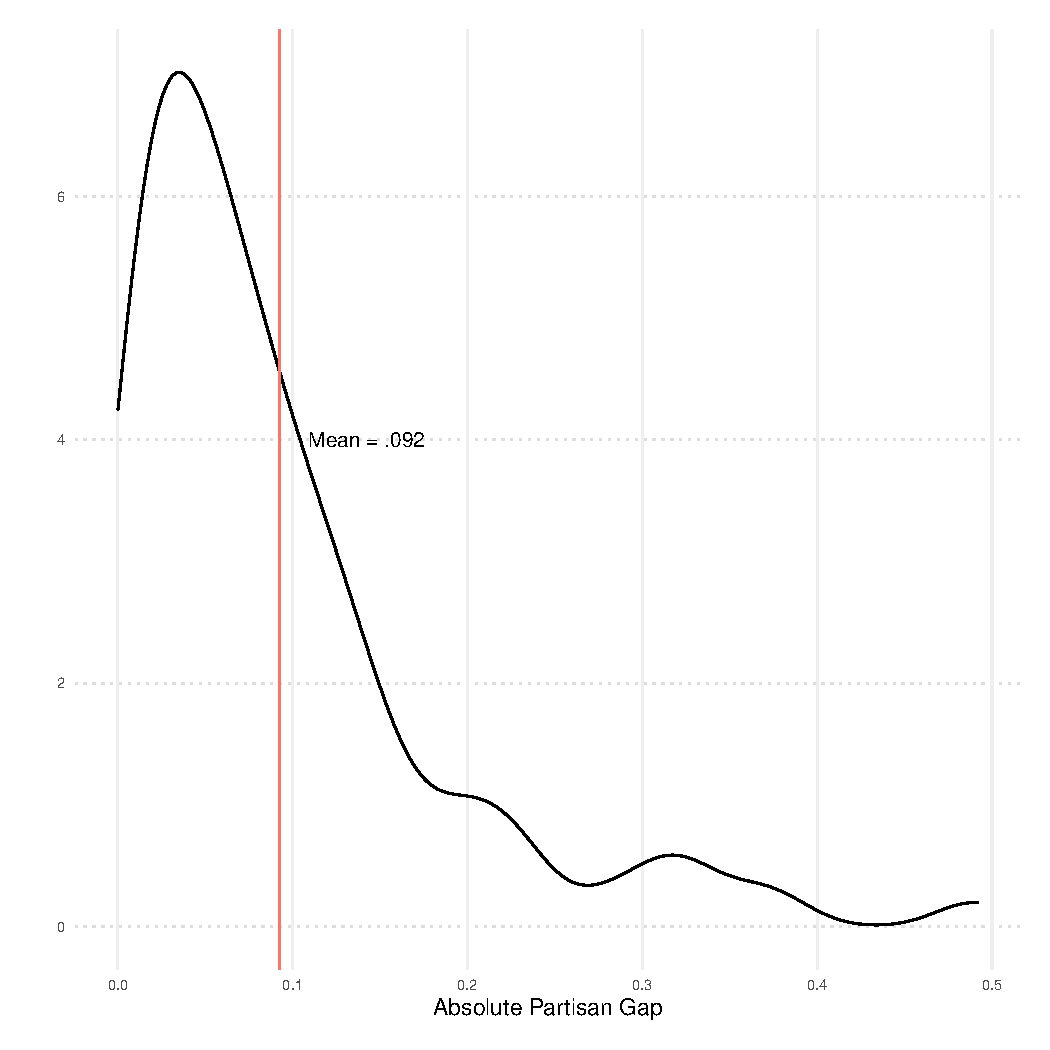
\includegraphics[scale=.8]{../figs/abs_value_p_gap.pdf}
   \caption*{Kernel density plot. \textit{n}=187.}
\end{figure}
\end{center}


\clearpage
\section{Additional ANES Information}

\subsection{Signed Partisan Gaps by Item - ANES Economic Retrospection Questions}
\label{append_econ}

% latex table generated in R 4.1.2 by xtable 1.8-4 package
% Sat Jan 01 21:26:39 2022
\begin{table}[!htb]
\centering
\caption{Partisan Gap on Economic Retrospection Items} 
\label{tab:econ}
\begingroup\tiny
\begin{tabular}{lllcccccc}
  \hline
Item & Study & Year & R & n(R) & D & n(D) & Signed Gap & $\textit{p(Gap)}$ \\ 
  \hline
Economy over past year & ANES & 1980 & 0.962 &  528 & 0.931 &  841 & 0.031 & 0.016 \\ 
  Economy over past year & ANES & 1982 & 0.530 &  445 & 0.758 &  774 & 0.228 & 0.000 \\ 
  Economy over past year & ANES & 1984 & 0.627 &  883 & 0.246 & 1063 & 0.381 & 0.000 \\ 
  Economy over past year & ANES & 1986 & 0.316 &  772 & 0.170 & 1088 & 0.146 & 0.000 \\ 
  Economy over past year & ANES & 1988 & 0.281 &  829 & 0.104 &  954 & 0.177 & 0.000 \\ 
  Economy over past year & ANES & 1990 & 0.958 &  714 & 0.954 & 1012 & 0.004 & 0.661 \\ 
  Economy over past year & ANES & 1992 & 0.080 &  927 & 0.024 & 1228 & 0.056 & 0.000 \\ 
  Economy over past year & ANES & 1994 & 0.329 &  749 & 0.366 &  834 & 0.036 & 0.131 \\ 
  Economy over the past year & ANES & 1996 & 0.260 &  654 & 0.482 &  895 & 0.222 & 0.000 \\ 
  Economy over past year & ANES & 1998 & 0.384 &  467 & 0.529 &  656 & 0.145 & 0.000 \\ 
  Economy over past year & ANES & 2000 & 0.262 &  680 & 0.492 &  888 & 0.230 & 0.000 \\ 
  Economy over past year & ANES & 2002 & 0.357 &  665 & 0.198 &  703 & 0.159 & 0.000 \\ 
  Economy over past year & ANES & 2004 & 0.426 &  479 & 0.101 &  585 & 0.325 & 0.000 \\ 
  Economy over past year & ANES & 2008 & 0.873 &  653 & 0.937 & 1364 & 0.064 & 0.000 \\ 
  Economy over past year & ANES & 2012 & 0.441 & 1993 & 0.824 & 3100 & 0.383 & 0.000 \\ 
  Economic condition of women over past year & ANES & 1984 & 0.543 &  875 & 0.411 & 1057 & 0.132 & 0.000 \\ 
  Economic condition of blacks over past year & ANES & 1984 & 0.388 &  872 & 0.283 & 1023 & 0.105 & 0.000 \\ 
  Economy since July 4th & ANES & 1992 & 0.730 &  857 & 0.575 & 1145 & 0.155 & 0.000 \\ 
  Economy compared to four years ago & ANES & 1992 & 0.756 &  857 & 0.856 & 1145 & 0.100 & 0.000 \\ 
  Economy since Clinton took office & ANES & 1998 & 0.646 &  468 & 0.839 &  659 & 0.193 & 0.000 \\ 
  Economy compared to 1992 & ANES & 2000 & 0.648 &  646 & 0.771 &  822 & 0.123 & 0.000 \\ 
  Economy compared to 2008 & ANES & 2016 & 0.214 & 1724 & 0.613 & 1936 & 0.399 & 0.000 \\ 
   \hline
\end{tabular}
\endgroup
\end{table}

\clearpage

\vspace{-3cm}
\subsection{Knowledge Question Wordings and Correct Answers - ANES Economic Retrospection Items}
\label{append_q_text_anes_econ}

\normalsize
{\begin{itemize}
\item \textbf{Economy better or worse over past year}\footnote{National economic conditions based on Federal Reserve Economic data (available at \begin{footnotesize} \url{fred.stlouisfed.org} \end{footnotesize}). The specific indicator is Real Gross Domestic Product per Capita, Quarterly, Seasonally Adjusted Rates, Chained to 2009 Dollars. To determine ``correct'' responses, we calculated the difference between real GDP per capita in Q3 in the year prior to the election and real GDP per capita in Q3 of the election year. Any difference with an absolute value of less than \$500 was coded as ''stayed about the same;'' anything above \$500 was coded as ``better,'' and anything less than \$500 was coded as ''worse.'' As noted in the manuscript, in calculating the signed partisan gap for these items, we did not change the sign of the partisan difference if the correct answer is coded as ''stayed about the same.''}   \\
Would you say that over the past year the nation's economy has gotten better, stayed\footnote{1984: ``about'' inserted here} the same or gotten worse?\footnote{An alternate version in 2002 reversed the direction of the options in the question.} 

\textit{Response options: Better, stayed [about] the same, gotten worse} \\

\begin{table}[H]
\centering
\caption{Economy over the past year - correct responses by year}
\vspace{.1in}
\label{econ_corr_by_year}
\begin{tabular}{ll}
\textbf{Year} & \textbf{Correct answer}       \\
1980 & Worse                 \\
1982 & Worse                 \\
1984 & Stayed about the same \\
1986 & Stayed the same \\
1988 & Stayed the same \\
1990 & Worse                 \\
1992 & Stayed the same \\
1994 & Better                \\
1996 & Better                \\
1998 & Stayed the same \\
1990 & Worse                 \\
1992 & Stayed the same \\
1994 & Better                \\
1996 & Better                \\
1998 & Stayed the same \\
2000 & Stayed the same \\
2002 & Worse                 \\
2004 & Stayed the same \\
2008 & Worse                 \\
2012 & Worse                 \\
2016 & Better               
\end{tabular}
\end{table}

   \end{itemize}}

\clearpage
\large \noindent{1984}

\begin{itemize}
\normalsize
\item \textbf{Economic condition of women over past year}\footnote{Economic condition of women based on subgroup unemployment figures from the Bureau of Labor Statistics (available at \url{data.bls.gov}). The specific indicator is Annual Unemployment Rates. To determine ``correct'' responses, we compared unemployment levels from previous year's annual average. (With the exception of 2008, in all years listed, unemployment did not change measurably---that is, by an increase or decrease of more than one third of one percentage point---over the course of the election year.) Unemployment was considered to have stayed ``about the same'' if it did not increase or decrease more than one third of one percentage point from the previous year.}   \\
What about women? Would you say that over the past year the economic position of women has gotten better, stayed about the same, or gotten worse? 
\textit{Response options: \textbf{Better}, stayed about the same, gotten worse} 
\end{itemize}

\normalsize
\begin{itemize}
\item \textbf{Economic condition of blacks over past year}\footnote{Economic condition of blacks based on subgroup unemployment figures from the Bureau of Labor Statistics (available at \url{data.bls.gov}). We follow our previous coding scheme for unemployment as described above.}   \\
Would you say that over the past year the economic position of blacks has gotten better, stayed about the same, or gotten worse?

\textit{Response options: \textbf{Better}, stayed about the same, gotten worse} 
\end{itemize}

\vspace{.1in}
\large \noindent{1992}
\normalsize
\begin{itemize}
\item \textbf{Economy compared to four years ago}\footnote{Economy compared to four years ago based on information chronicled in \citet{hershey_1993}.}   \\
Compared to four years ago, would you say that the nation's economy has gotten better, stayed about the same, or gotten worse?        \\
\textit{Response options: Gotten better, stayed about the same, \textbf{gotten worse}} 
\end{itemize}

\normalsize
\begin{itemize}
\item \textbf{Economy since July 4th}\footnote{Economic information since July based on information chronicled in \citet{apple_1992}.}   \\
What about in the last few months, since about the 4th of July. Would you say that the nation's economy has gotten better, stayed about the same, or gotten worse?    \\
\textit{Response options: \textbf{Gotten better}, stayed about the same, gotten worse} 
\end{itemize}
\vspace{.1in}

\large \noindent{1998}
\normalsize
\begin{itemize}
\item \textbf{Economy since Clinton took office}\footnote{Economy better/worse based on Federal Reserve Economic data (available at \url{fred.stlouisfed.org}). The specific indicator is Real Gross Domestic Product per Capita, Quarterly, Seasonally Adjusted Rates, Chained to 2009 Dollars. To determine the ``correct'' response, we calculated the difference between real GDP per capita in Q1 of 1993 and real GDP per capita in Q3 of 1998. We also checked the quarterly data between these endpoints to ensure the indicator trended upward.} \\
Would you say that since Clinton took office, the nation's economy has gotten better, stayed about the same, or gotten worse?           \\
\textit{Response options: \textbf{Gotten better}, stayed about the same, gotten worse} \\
\end{itemize}

\large \noindent{2000}
\normalsize
\begin{itemize}
\item \textbf{Economy compared to 1992}\footnote{Economy better/worse based on Federal Reserve Economic data (available at \url{fred.stlouisfed.org}). The specific indicator is Real Gross Domestic Product per Capita, Quarterly, Seasonally Adjusted Rates, Chained to 2009 Dollars. To determine the ``correct'' response, we calculated the difference between real GDP per capita in Q1 of 1993 and real GDP per capita in Q3 of 2000. We also checked the quarterly data between these endpoints to ensure the indicator trended upward.} \\
Since 1992, would you say President Clinton has made the nation's economy better, made the economy worse, or had no effect on the economy one way or the other?        \\     
\textit{Response options: \textbf{Made the economy better}, made the economy worse, no effect} \\
\end{itemize}


\large \noindent{2016}

\normalsize
\begin{itemize}
\item \textbf{Economy compared to 2008}\footnote{Economy better/worse based on Federal Reserve Economic data (available at \url{fred.stlouisfed.org}). The specific indicator is Real Gross Domestic Product per Capita, Quarterly, Seasonally Adjusted Rates, Chained to 2009 Dollars. To determine the ``correct'' response, we calculated the difference between real GDP per capita in Q3 of 2008 and real GDP per capita in Q3 of 2016. We also checked the quarterly data between these endpoints to ensure the indicator trended upward.} \\
Would you say that compared to 2008, the nation's economy is now better, worse, or about the same?  \\     
\textit{Response options: \textbf{Better}, worse, about the same} \\
\end{itemize}

\clearpage



\clearpage




\end{document}